\documentclass[
  a4paper,
  abstract=true,
  twoside,
  listof=totoc,
  numbers=noenddot,
  bibliography=totoc,
  BCOR=1.5cm,
  headsepline,
  DIV=12,
  appendixprefix,
  final
] {tudscrreprt}

% You should select either american or british instead of english here:
\usepackage[ngerman,english]{babel}
\usepackage{fontspec}

\usepackage[citebordercolor={0.75 0.75 1},
filebordercolor={0.75 0.75 1},
linkbordercolor={0.75 0.75 1},
% pagebordercolor={0.75 0.75 1},
urlbordercolor={0.75 0.75 1},
pdfborder={0.75 0.75 1},
hidelinks,
plainpages=false,pdfpagelabels=true]{hyperref}
\hypersetup{%
  pdftitle={Load Balancing in the L4Re Operating System Framework},
  pdfauthor={Paul Franitza},
  pdfkeywords={Operting Systems, Load Balancing, Scheduling},
}

% You can choose style "numeric" instead which is common in many papers.
% Without "maxbibnames=99" the bibliography entries only contain "First Name et al."
\usepackage[backend=biber,style=alphabetic,alldates=long,maxbibnames=99]{biblatex}

% FONT SETTINGS & ENCODING
% By default this build setup uses lualatex which supports special characters
% (öäüß<>) out of the box. If you ever want to switch to pdflatex but also
% keep the support for lualatex, add these three packages:
% \usepackage[T1]{fontenc}
% \usepackage[utf8]{luainputenc}
% \usepackage{lmodern}

\usepackage[nospace]{varioref}           % nice refs
\usepackage{csquotes}
\usepackage{graphicx}           % graphics
\usepackage{caption}            % manipulate fugures
\usepackage{subcaption}         % allow for subfigures
% Also checkout "minted" instead of "listings" - looks much nicer and supports
% more languages but requires "pygmentize" to be available on the command line
\usepackage{listings}           % nice source code listings
\usepackage{xcolor}
\usepackage{booktabs}           % nice tables
\usepackage{microtype}          % better looking text borders
\usepackage{siunitx}            % unified way of setting values with units
\usepackage{array}
\usepackage{fancybox}           % provide nice boxes
\usepackage{fancyvrb}           % algorithm-boxes
\usepackage{pdfpages}
\usepackage{hyphenat}
\usepackage{todonotes}
\usepackage{xspace}
\usepackage{setspace}

% --- OWN ---

\usepackage{pgfplots}
\usepgfplotslibrary[groupplots]
\pgfplotsset{compat=1.18}
%\usepgfplotslibrary{external}
%\tikzexternalize
\usepackage[dvipsnames]{xcolor}
\usepackage{colortbl}
\usepgfplotslibrary{statistics}
\usepackage[toc,page]{appendix}
\usepackage{nth}
\usepackage{threeparttable}

% use this one last
% (redefines some macros for compatibility with KOMAScript)
\usepackage{scrhack}

\addbibresource{own.bib}
\input{preamble/color.tex}
% Biblatex Style
\setcounter{secnumdepth}{3}     % limit enumeration depth
\setcounter{tocdepth}{1}        % limit TOC depth

% Listing Style

\lstset{ %
    frame=shadowbox,
    rulesepcolor=\color{blue},
    backgroundcolor=\color{white},   % choose the background color; you must add \usepackage{color} or \usepackage{xcolor}
    %  basicstyle=\footnotesize,        % the size of the fonts that are used for the code
    breakatwhitespace=false,         % sets if automatic breaks should only happen at whitespace
    breaklines=true,                 % sets automatic line breaking
    captionpos=b,                    % sets the caption-position to bottom
    commentstyle=\color{mygreen},    % comment style
    deletekeywords={...},            % if you want to delete keywords from the given language
    escapeinside={\%*}{*)},          % if you want to add LaTeX within your code
    extendedchars=true,              % lets you use non-ASCII characters; for 8-bits encodings only, does not work with UTF-8
    frame=single,                    % adds a frame around the code
    keepspaces=true,                 % keeps spaces in text, useful for keeping indentation of code (possibly needs columns=flexible)
    keywordstyle=\color{blue},       % keyword style
    language=C,                 % the language of the code
    % morekeywords={*,...},            % if you want to add more keywords to the set
    numbers=left,                    % where to put the line-numbers; possible values are (none, left, right)
    numbersep=7pt,                   % how far the line-numbers are from the code
    numberstyle=\tiny\color{mygray}, % the style that is used for the line-numbers
    rulecolor=\color{black},         % if not set, the frame-color may be changed on line-breaks within not-black text (e.g. comments (green here))
    showspaces=false,                % show spaces everywhere adding particular underscores; it overrides 'showstringspaces'
    showstringspaces=false,          % underline spaces within strings only
    showtabs=false,                  % show tabs within strings adding particular underscores
    stepnumber=1,                    % the step between two line-numbers. If it's 1, each line will be numbered
    stringstyle=\color{mymauve},     % string literal style
    tabsize=2,                       % sets default tabsize to 2 spaces
    title=\lstname                   % show the filename of files included with \lstinputlisting; also try caption instead of title
}

% Typesetting options
\tolerance 2414
\hbadness 2414
\emergencystretch 1.5em
\hfuzz 0.3pt
\widowpenalty=10000     % Hurenkinder
\clubpenalty=10000      % Schusterjungen
\vfuzz \hfuzz
\raggedbottom

% use nice footnote indentation
\deffootnote[1em]{1em}{1em}{\textsuperscript{\thefootnotemark}\,}

% ########################################################

% - Roman/Serif font for all headings.
%   Default is sans-serif which looks kind of unprofessional with the default font family.
% - Packages like titlesec don't work well together with KOMA
% - "disposition" means, that this setting is for all headings (chapter level, section level, ...)
%   see: https://mirror.physik.tu-berlin.de/pub/CTAN/macros/latex/contrib/koma-script/doc/scrguide.pdf
\addtokomafont{disposition}{\rmfamily}

% --- OWN ---
\pgfplotsset{
	baseline boxplot/.style = {
		boxplot/draw direction = y,
		boxplot/whisker range  = 1.5,
		xtick                  = \empty,
		ymajorgrids            = true,
		height 				   = 5.8cm,
		width				   = 8cm,
		legend columns         = -1,
		legend to name         = boxplotlegend,
		legend style           = {font=\small},
	}
}

\pgfplotsset{
	cpu plot/.style = {
		ybar,
		ymajorgrids = true,
		bar width = 5pt,
		width = 0.485\linewidth, height = 7cm,
		symbolic x coords = {2, 4, 8},
		xtick = data,
		xlabel = {CPUs},
		enlarge x limits = 0.25,
		legend style = {legend columns=3, font=\footnotesize}
	}
}

\pgfplotsset{
	para plot/.style = {
		ybar,
		ymajorgrids = true,
		bar width = 5pt,
		width = 0.485\linewidth, height = 7cm,
		symbolic x coords = {Under, Full, Over},
		xtick = data,
		xlabel = {Load},
		enlarge x limits = 0.25,
		legend style = {legend columns=3, font=\footnotesize}
	}
}

\pgfplotsset{
	overhead plot/.style = {
		grid = major,
		width = 11.2cm, height = 4.3cm,
		xtick = {10,100,500,1000,2000},
		ymin = 0,
		xmin = 10,
		xmax = 2000,
	}
}


% some common commands
\newcommand{\drops}{\texorpdfstring{\textsc{Drops}\xspace}{DROPS}}
\newcommand{\LLinux}{\texorpdfstring{L$\!^4$Linux}{L4Linux}}

\newcommand{\NOVA}{NOVA\xspace}
\newcommand{\QEMU}{QEMU\xspace}

% #1 = value to display, #2 = same value (numeric), #3 = value of the paired row
\newcommand{\cmpcell}[3]{%
	\pgfmathsetmacro{\diffpct}{(#2-#3)/#3*100}
	\pgfmathsetmacro{\intensity}{min(abs(\diffpct)*4, 80)}
	\pgfmathparse{\diffpct > 0 ? 1 : 0}
	\ifnum\pgfmathresult=1
	\cellcolor{Red!\intensity}
	\else
	\cellcolor{Green!\intensity}
	\fi
}

% If you know when you will hand in your thesis, enter the date here.
%\date{30. April 2009}
%\newcommand{\printdate}{\@date}

\begin{document}

\pagenumbering{Roman}

\selectlanguage{english}

\begin{singlespace}

    % Depending on the thesis that you are writing, choose the proper setting here
    \subject{diploma} % for Diploma Thesis
    \graduation[Dipl.-Inf.]{Diplom-Informatiker}
    % \subject{master} % for Master Thesis
    % \graduation[M.Sc.]{Master of Science}
    % \subject{bachelor} % for Bachelor Thesis
    % \graduation[B.Sc.]{Bachelor of Science}
    % \subject{evidence} % for Student Research Project (Großer Beleg)

    \title{Load Balancing in the L4Re Operating System Framework}

    \author{%
        Paul Franitza%
        \matriculationnumber{5009939}%
        \dateofbirth{November 25, 2001}%
        \placeofbirth{Duisburg}%
    }

    \date{\today} % \printdate % if you defined date earlier

    % English version
    \faculty{Faculty of Computer Science}
    \institute{Institute of Systems Architecture}
    \chair{Chair of Operating Systems}
    % German version
    %\faculty{Fakultät Informatik}
    %\institute{Institut für Systemarchitektur}
    %\chair{Professur für Betriebssysteme}

    \professor{Prof.\ Dr.-Ing.\ Horst Schirmeier}
    \supervisor{Dr.-Ing.\ Adam Lackorzynski}

    \maketitle
\end{singlespace}

\cleardoublepage


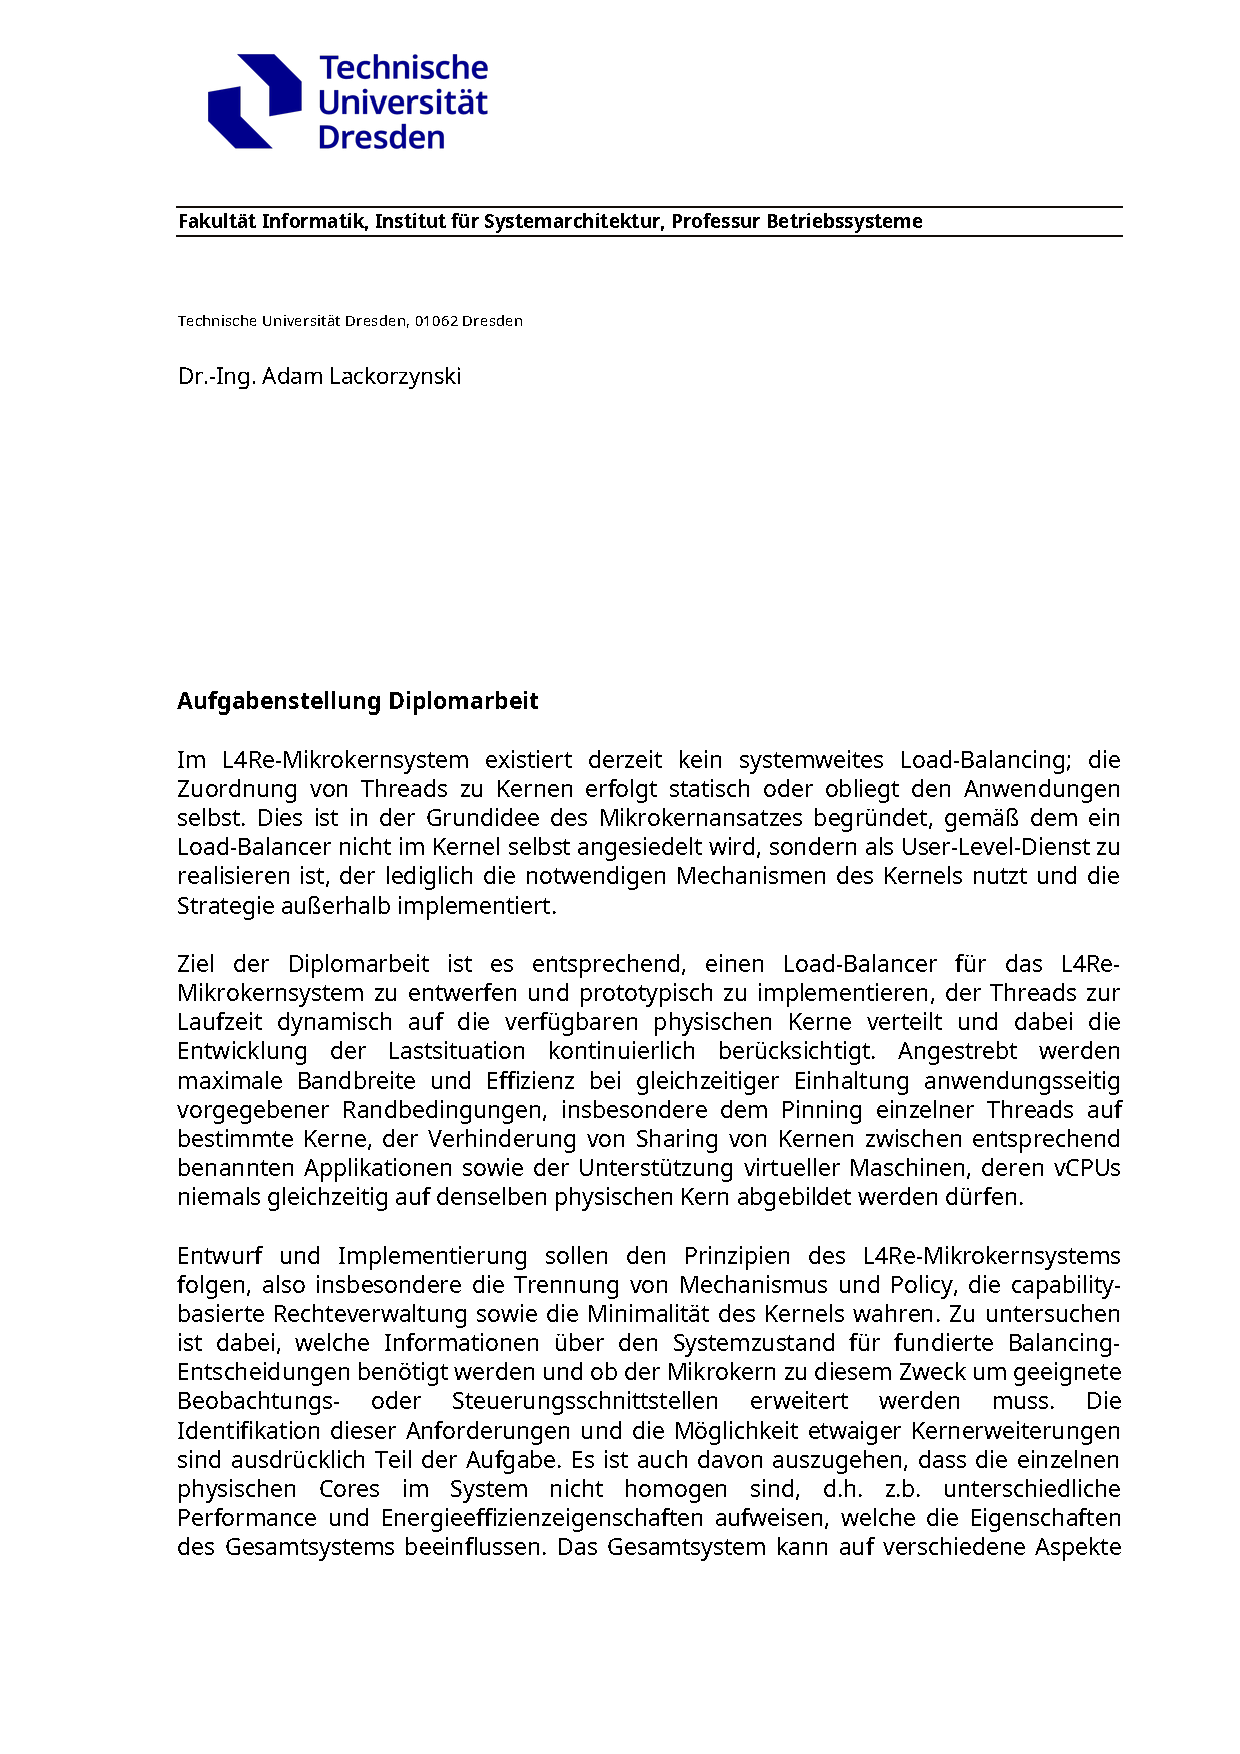
\includepdf[pages={1-}]{images/diplom-aufgabe-paul-franitza.pdf}

\cleardoublepage

%\selectlanguage{english}

%\section*{\vfill{} \thispagestyle{empty}
%Selbstständigkeitserklärung}
\section*{\vfill{} \thispagestyle{empty}
Statement of authorship}

%Hiermit erkläre ich, dass ich diese Arbeit selbstständig verfasst
%und keine anderen als die angegebenen Quellen und Hilfsmittel benutzt habe.
I hereby certify that I have completed this work on my own and without the
help of anything other than the indicated sources and resources.
\bigskip{}

\noindent Dresden, \today % \printdate % if you defined date earlier
\vspace{2.5cm}

\noindent Paul Franitza \cleardoublepage{}


% NOTE: if you selected british or american above, change that here too
\selectlanguage{english}

\begin{abstract}
% -*- Mode: Latex -*-

%  Zusammenfassung

% Zu einer runden Arbeit gehört auch eine Zusammenfassung, die
% eigenständig einen kurzen Abriß der Arbeit gibt. Eine halbe bis ganze
% DINA4 Seite ist angemessen. Dafür läßt sich keine Gebrauchsanweisung
% geben (für irgendetwas müssen die Betreuer ja auch noch da
% sein).

Modern hardware increasingly combines processor cores of varying types and speeds on a single chip (asymmetric multiprocessing, or AMP).
However, the L4Re operating system framework does not provide CPU load balancing.
Threads need to be statically assigned to cores by the applications themselves.
This approach aligns with the microkernel philosophy of separating mechanism from policy, but it leaves the question of AMP-aware, dynamic thread placement unaddressed.

This thesis proposes a user-level load balancing service for L4Re on x86-64 that distributes threads across physical cores during runtime.
It respects application-supplied constraints, such as thread pinning, core-sharing restrictions, and the placement requirements of virtual machine vCPUs.
The design adheres to L4Re's proxy pattern: a scheduling proxy intercepts scheduler calls, per-CPU monitoring threads track system state, and a commander thread performs periodic rebalancing based on virtual load (vload), a preemption-based metric capturing both CPU utilization and saturation.
AMP awareness is achieved by scaling the vload of each CPU according to its measured compute performance.
Realizing the design required extending the L4Re microkernel with three new interfaces for capability comparison, thread probing, and pinned scheduling.

The resulting load balancer is evaluated against the Linux EEVDF scheduler using ported CPU-bound benchmarks across baseline, scalability, and parallel-load scenarios while its own monitoring overhead is measured directly.
It is imperative to implement periodic rebalancing procedures, as a non-rebalancing variant trails by a factor of two to four due to a pile-on effect from stale load information.
The rebalancing configurations remain within a narrow range of each other, irrespective of the monitoring interval.
They introduce a monitoring overhead of less than 1\,\% and approach EEVDF's throughput within approximately 2--7\,\% percent.
This demonstrates that AMP-aware load balancing is achievable as a policy-separated userland service at a modest cost relative to a mature monolithic scheduler.

%%% Local Variables:
%%% TeX-master: "diplom"
%%% End:



\end{abstract}

\cleardoublepage

\addchap{Acknowledgments}
\label{sec:acknowledgments}

I would like to express my sincere appreciation to my supervisor, Dr.-Ing.\ Adam Lackorzynski, for constant feedback, numerous discussions in which we both had the opportunity to elaborate on our thoughts, and proofreading this thesis.

I would also like to thank my colleagues Matthias Lange, Steffen Liebergeld, Jan Klötzke, Georg Kotheimer, and Dr.-Ing.\ Frank Mehnert for proofreading, discussing design choices with me, and patiently explaining topics I was less familiar with.

Special thanks go to Philipp Eppelt, whose door was always open for quick conversations and feedback whenever I was indecisive about an idea.
These conversations also helped me understand the bigger picture of what writing a thesis actually involves and grounded me in reasonably planning the time this work required.

I am grateful to my family and friends for their support and the genuine interest they showed in what I was working on throughout the development and writing of this thesis.
In particular, I want to thank Elli and Diana for their emotional support during challenging stretches and Paulus for helping me to greatly improve the visual appearance of this thesis.

\cleardoublepage

%%% Local Variables:
%%% TeX-master: "diplom"
%%% End:


\cleardoublepage

\tableofcontents

\cleardoublepage

\listoffigures

\begingroup
	\let\clearpage\relax
	\vspace{-1cm}
	\listoftables
\endgroup

\cleardoublepage

\pagenumbering{arabic}
% use \input for small stuff (like a list you include twice or a tiks figure)
% and \include for large latex compilation workloads (like a chapter) to get faster builds.
\chapter{Introduction}
\label{sec:intro}

% Die Einleitung schreibt man zuletzt, wenn die Arbeit im Großen und
% Ganzen schon fertig ist. (Wenn man mit der Einleitung beginnt - ein
% häufiger Fehler - braucht man viel länger und wirft sie später doch
% wieder weg). Sie hat als wesentliche Aufgabe, den Kontext für die
% unterschiedlichen Klassen von Lesern herzustellen. Man muß hier die
% Leser für sich gewinnen. Das Problem, mit dem sich die Arbeit befaßt,
% sollte am Ende wenigsten in Grundzügen klar sein und dem Leser
% interessant erscheinen. Das Kapitel schließt mit einer Übersicht über
% den Rest der Arbeit. Meist braucht man mindestens 4 Seiten dafür, mehr
% als 10 Seiten liest keiner.

The parallel execution of tasks was a problem in the past, and it remains so throughout the present day.
Imagine two checkout lanes running next to each other.
One serves customer by customer slowly but steadily, while the other empties out twice as fast.
The staff have different working speeds, the clients have varying numbers of items in their carts, and the cashier queues have differing lengths.
All those conditions lead to one usually choosing a suboptimal line for being processed as fast as possible.
A similar situation was experienced in the early \nth{20} century by telephone exchange centers.
Calls arrived at random, each one occupied a line for an arbitrary duration, and only a finite number of lines were available.
Additionally, each needed to be staffed by an operator.
The task the Danish mathematician Agner Krarup Erlang was faced with when working at the Copenhagen Telephone Company was how many circuits and operators the exchange needed for an expected volume of traffic while keeping the probability of a blocked call below an acceptable threshold.
As hold queues did not yet exist, callers were simply turned away when every line was occupied.
Hence, the goal was to minimize the number of blocked calls and, later, to reduce the waiting time in a hold queue as far as possible.
To solve those problems, Erlang introduced the field of queueing theory modeling such systems.\\

Time advanced, and so did technology, but the problems remained.
While modern telecommunication has since solved the problem for exchange centers as calls are now routed digitally, without manual operation, picking a checkout queue remains a task every customer still has to solve alone.

Further, this abstraction carries over almost directly into computing. A single processor core working through a stream of incoming tasks is structurally identical to a checkout lane with one cashier.
The jobs arrive, occupy the core for a finite duration, and are served in some order.
This uniprocessor case is well understood because decades of operating systems research have produced reliable scheduling strategies from round-robin to multilevel feedback queues.
They answer the question of who runs next when there is exactly one queue and one server.

The introduction of multiple processor cores changed comparatively little at first.
Several identical cores amount to several identical checkout lanes.
They are uniform in speed, each equally suited to any job.
Distributing work across them stays close to the classical queuing problem, where a job, like a customer, needs only be routed to whichever lane is shortest or fastest to clear.

\begin{figure}[h]
	\centering
	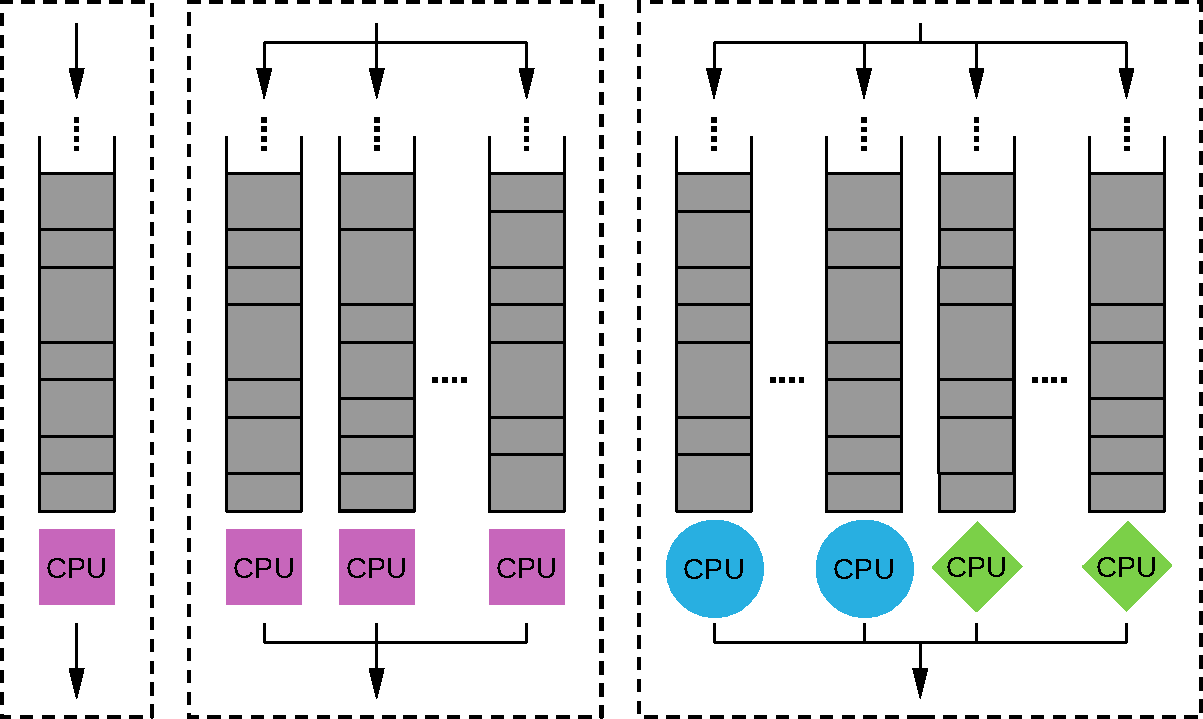
\includegraphics[width=0.75\textwidth]{images/queue_processing.pdf}
	\caption{Three queuing configurations: a single server (left), multiple servers of uniform speed (center), and multiple servers of asymmetric speed (right), illustrating the transition from uniprocessor to heterogeneous architecture scheduling.}
	\label{fig:queue-processing}
\end{figure}

This assumption of uniformity breaks down with modern processor chips. Contemporary hardware increasingly combines cores of different sizes and speeds on a single chip, so-called heterogeneous multiprocessing.
Doing so trades uniform performance for energy efficiency and workload-specific throughput.
Just as an operator once decided which caller was connected to which line, it is now the operating system's task to decide which job is assigned to which core.
Every incoming job must be routed not merely to any free queue, but to the queue best suited to both the job and the current state of the system.
This decision needs to be made anew for every single job rather than once for the system as a whole.
Unlike a shopper, the operating system cannot simply glance down the line and estimate how long a job will take.
It must decide under incomplete information, and unlike a customer changing lanes, moving a job from one queue to another is never free.\\

Queueing theory already distinguishes between two such decisions, even if the checkout analogy blurs them together.
It separates the question of who is served next within a line from the question of which line a new arrival should join.
The former defines the field of scheduling theory, and within an operating system, the component concerned with this decision is called a scheduler.
The latter is usually a subsystem of the scheduler, and its task is to balance load across the system; hence, the name load balancing.
As core responsibilities of every operating system, both must be designed to meet the demands of the workloads they serve.
This thesis is not about how work is ordered for a single server but about the strategy that distributes work among the available processing units.
Load balancing can pursue different goals, among them throughput, responsiveness, energy efficiency, and fairness.
Because these goals often conflict, a careful choice must be made before any implementation begins.
Designing such a balancing component becomes notably harder in microkernel-based operating systems, a challenge this thesis returns to once the relevant architectural background has been introduced.
Concretely, this thesis develops and evaluates a load-balancing component for the L4Re microkernel's userland that is aware of heterogeneous architecture, making the following contributions:

\begin{itemize}
	\item Design and implementation of a load balancing component for the L4Re userland
	\item Investigation of metrics suited to balancing load across heterogeneous cores
	\item Extension of L4Re microkernel interfaces where required by the design
	\item Selection of benchmarks, development of a benchmarking harness, and construction of dedicated test cases
	\item Evaluation of multiple load balancer configurations against Linux's EEVDF scheduler
\end{itemize}

\section{Outline}

This work is structured as follows.
Chapter~\ref{sec:state} introduces the terminology used throughout the thesis and surveys related work on load balancing in general-purpose, AMP, and microkernel-based operating systems. It then examines microkernel architecture in more depth, covering inter-process communication, scheduling, and heterogeneous hardware.
Chapter~\ref{sec:design} presents the design of the load balancing component developed in this thesis, including an architectural overview of its key components, their behavior, and how the design accounts for the constraints of the underlying microkernel architecture.
Chapter~\ref{sec:implementation} discusses challenges encountered during the implementation, extends the design with concepts from distributed systems, and describes tested optimizations.
Chapter~\ref{sec:evaluation} evaluates the resulting load balancer, comparing multiple configurations of the service against the Linux EEVDF scheduler on a set of selected benchmarks and purpose-built test cases.
Chapter~\ref{sec:futurework} outlines directions for extending, investigating, and optimizing the developed system, and Chapter~\ref{sec:conclusion} closes the thesis with a conclusion.

\cleardoublepage

%%% Local Variables:
%%% TeX-master: "diplom"
%%% End:

\chapter{Technical Background}
\label{sec:state}

% Hier werden zwei wesentliche Aufgaben erledigt:

% 1. Der Leser muß alles beigebracht bekommen, was er zum Verständnis
% der späteren Kapitel braucht. Insbesondere sind in unserem Fach die
% Systemvoraussetzungen zu klären, die man später benutzt. Zulässig ist
% auch, daß man hier auf Tutorials oder Ähnliches verweist, die hier auf
% dem Netz zugänglich sind.

% 2. Es muß klar werden, was anderswo zu diesem Problem gearbeitet
% wird. Insbesondere sollen natürlich die Lücken der anderen klar
% werden. Warum ist die eigene Arbeit, der eigene Ansatz wichtig, um
% hier den Stand der Technik weiterzubringen? Dieses Kapitel wird von
% vielen Lesern übergangen (nicht aber vom Gutachter ;-), auch später
% bei Veröffentlichungen ist "Related Work" eine wichtige Sache.

% Viele Leser stellen dann später fest, daß sie einige der Grundlagen
% doch brauchen und blättern zurück. Deshalb ist es gut,
% Rückwärtsverweise in späteren Kapiteln zu haben, und zwar so, daß man
% die Abschnitte, auf die verwiesen wird, auch für sich lesen
% kann. Diese Kapitel kann relativ lang werden, je größer der Kontext
% der Arbeit, desto länger. Es lohnt sich auch! Den Text kann man unter
% Umständen wiederverwenden, indem man ihn als "Tutorial" zu einem
% Gebiet auch dem Netz zugänglich macht.

% Dadurch gewinnt man manchmal wertvolle Hinweise von Kollegen. Dieses
% Kapitel wird in der Regel zuerst geschrieben und ist das Einfachste
% (oder das Schwerste weil erste).

This chapter will introduce the basic terminology used throughout this work, followed by the related work done in the field of load balancing, and close with a deeper dive into technical concepts reoccurring in Chapter~\ref{sec:design} and Chapter~\ref{sec:implementation}.
Starting with the terminology used throughout this thesis, followed by the related work done in the fields of load balancing and closing with an explanation of the most important topics.

\section{Terminology}

\paragraph{Central Processing Unit (CPU).}
A CPU is the hardware unit that executes an instruction stream.
CPUs or hardware threads are referred to by a logical number, denoted by CPU<N>.

\paragraph{Thread.}
A thread is a schedulable unit of execution.
It contains the state of the execution of a program, like the program counter, stack pointer, and registers, and it is assigned to exactly one CPU at a time.

\paragraph{Virtual CPU (vCPU).}
A vCPU is a kernel abstraction that makes a thread behave like a physical CPU toward the user level.
Events such as interrupts, exceptions, and inter-process communication (IPC, see Section~\ref{sec:ipc}) are delivered asynchronously to a user-level entry point instead of blocking the thread.
It is, therefore, the basis for user-level schedulers and virtual machine monitors.

\paragraph{User-level Thread Control Block (UTCB).}
The User-level Thread Control Block is a small per-thread memory area shared between kernel and user space.
It holds the message registers used for IPC and further thread state that can thus be accessed without a system call.

\paragraph{Floating Point Unit (FPU).}
The FPU is the processor unit for floating-point arithmetic and has its own register set, which forms part of a thread's context. Its state is tracked per CPU and switched either lazily or eagerly.

\paragraph{Components.}
Components are the user-level programs the system is composed of, such as servers, device drivers, and applications.
Each of them runs isolated in its own address space and interacts with the others solely by IPC.

\paragraph{Capability.}
A capability is an unforgeable reference to a kernel or server object, stored in a slot of the task's capability table together with the rights it grants.
A thread can only communicate with objects for which it holds a capability.

\paragraph{Interface.}
An interface is the set of operations an object offers to its clients, invoked via IPC through a capability.
A client only depends on the interface, not on whether the object is implemented in the kernel or in a user-level server.

\paragraph{Proxy.}
A proxy is an object that implements the same interface as another object and forwards invocations to it.
Because clients cannot distinguish it from the original object, it can be interposed transparently to observe, delay, or redirect requests and enforce a policy.

\paragraph{Kernel and User Mode.}
Kernel mode is the privileged processor mode in which the microkernel runs with unrestricted access to the hardware.
All other software runs in the deprivileged user mode.
Crossing this boundary requires a trap into the kernel, making system calls comparatively expensive.

\paragraph{Run Queue.}
The run queue is the per-CPU kernel data structure that holds all threads that are ready to execute, usually ordered by a kind of priority metric.
The scheduler selects the next thread to run from it, which makes its occupancy a direct indicator of the load on that CPU.

\paragraph{Kip Clock.}
The Kernel Info Page (KIP) is a read-only page mapped into every task.
Its clock field contains a monotonically increasing time value in microseconds since boot.
It provides user-level code with timestamps without the cost of a system call at the resolution given by the kernel's timer configuration.

\paragraph{Software Interrupt Requests (IRQ).}
An IRQ object is a kernel object used for asynchronous notification.
A software IRQ is not bound to a hardware source but is triggered by user-level code, which allows one component to signal another without a blocking IPC.

\paragraph{Moe and the In Task Service (ITAS).}
Moe is the root task; it is the first user-level program started by the L4Re microkernel and provides the basic L4Re services such as data spaces, region maps, and name spaces.
ITAS is the event handler thread that is loaded into every application's address space, where it acts as a region manager, pager, and exception handler for that application.

\section{Related Work}

\subsection{General Purpose Scheduling}

This section will cover the Linux and Windows as representatives for general purpose scheduling in monolithic operating systems.
The Linux completely fair scheduler (CFS) and its successor, earliest eligible virtual deadline first (EEVDF), share the same load-balancing strategy, as their differences are located in core local scheduling decisions.
The utilization of a CPU is determined by the threads and thread groups located on that CPU via per-entity load tracking (PELT)~\cite{linux-internals-loadbalancing}.
Load balancing is triggered periodically, on idle CPUs and on thread wake/create events.
Linux employs scheduling domains that are then balanced by one designated CPU that can migrate up to 32 threads at a time between the busiest and idlest scheduling groups.
The domains are organized in a topology that is balanced from the bottom up.
Additionally, imbalance thresholds scaling with distance and cache-locality heuristics are used on non-uniform memory access (NUMA) systems, limiting unnecessary migrations~\cite{wasted_cores, cfs_vs_ule}.

Windows follows a pull-based approach where idle processors search for work and try to steal it instead of busy ones pushing it away.
In contrast to Linux, no periodic rebalancing is executed, but rather on-demand when the placement logic finds a better CPU.
The thread placement employs a hierarchical fallback order based on simultaneous multithreading (SMT) topology: ideal (assigned at thread creation time), last, current, same-SMT-set, and lowest-numbered CPU to preserve cache locality.
NUMA and SMT awareness are provided by proactive migrations at the quantum end when a thread's SMT set is busy while ideal nodes remain idle~\cite{windows_internals, clr_inside_out}.

Both designs are mechanism-rich with the advantage of having all scheduling information without any overhead because of the monolithic operating system design.
The microkernel philosophy prohibits such behavior, as a load balancer residing in userland cannot have detailed information about the whole system state right away but needs to obtain it from the kernel via a dedicated interface.

\subsection{AMP Aware Load Balancing}

Asymmetric multiprocessing (AMP) awareness describes the ability of a balancing system to have knowledge about the processor architecture underneath and use it to make informed decisions.
The work of Li \textit{et al.}~\cite{faster-core-first} extended the Linux CFS with AMPS to harness asymmetric multi-core architectures (see Section~\ref{sec:amp}).
To overcome the differences in performance and efficiency cores, they presented three concepts.
First, scaling the CPU load by its compute power, populating fast cores first, a policy known as \enquote{faster core first}; and finally, gating migrations by NUMA and cache-miss cost prediction.
Although a minimal patch to CFS, it still sits on top of a monolithic scheduler, contrasting a from-scratch design followed through in this thesis.

Shelepov and Saez \textit{et al.}~\cite{hass-scheduling} took an offline approach with Heterogeneous Awareness Scheduling (HASS) on OpenSolaris, avoiding runtime overhead entirely by matching threads to core types via architectural signatures collected in advance and used to predict per-core completion time.
HASS achieves performance comparable to an omniscient static assignment, but the reliance on offline profiling means it cannot react to shared-cache contention or a thread's phase changes at runtime.
The authors previously explored a dynamic load-balancing approach but found that HASS's offline profiling outperformed it.
The static-vs-dynamic trade-off this exposes is directly relevant to a design that instead derives its load signal from the kernel's own runtime state.

Koufaty, Reddy, and Hahn~\cite{bias-scheduling} took a lighter-weight, fully online approach with bias scheduling, classifying each thread's preference for big or small cores from internal versus external stall counters already present in hardware.
They apply the classification only at the point of load balancing rather than continuously.
Their evaluation is notable for modeling heterogeneity through distinct core microarchitectures rather than the frequency-scaled cores common in earlier work.
Additionally, they show that DVFS-based emulation of heterogeneity produces significantly different behavior from real asymmetric cores.
The low-overhead, existing-counter-based metric is conceptually close to the online concepts used in this thesis, even though bias scheduling still classifies threads only coarsely rather than estimating cross-core performance directly.

Van Craeynest \textit{et al.}~\cite{pie} pushed the estimation further with Performance Impact Estimation (PIE), predicting cross-core performance from a thread's cycles per instruction stack together with its memory- and instruction-level parallelism rather than sampling actual execution on the other core type.
PIE improves prediction accuracy over both sampling- and bias-based approaches at a hardware cost the authors report as roughly 15 bytes of additional per-core hardware state, but this comes at the price of a considerably more elaborate estimation model.
Where PIE trades metric simplicity for prediction accuracy, this thesis takes the opposite position, favoring a simple, directly observable metric over a modeled estimate of cross-core performance.

\subsection{Microkernel Load Balancing}

QNX's AMP support forgoes runtime load balancing altogether: CPU-to-process binding is fixed at boot time, and the vendor documentation explicitly characterizes dynamic migration as impractical given the cost of checkpointing and interrupting a running process~\cite{qnx-amp}.
Notably, QNX's use of the term \enquote{AMP} differs from the hybrid-core sense used in this thesis, as it also covers configurations running entirely different operating systems per core rather than cores of a single ISA with different performance characteristics.
QNX, therefore, represents something close to a null case among the related work, showing the motivation for a dynamic, AMP-aware balancer in a microkernel setting.

The seL4-derived balancer described in~\cite{global-dynamic-load-balancing} is one of the few load-balancing designs implemented directly for a microkernel rather than retrofitted onto a monolithic scheduler.
It follows a centralized design in which load is computed as the summed remaining time slices of ready threads per core and compared against a static twenty percent imbalance threshold, with rebalancing triggered both on thread creation and by a 100\,\si{\ms} periodic timer, migrating a thread only if doing so strictly improves the balance.
The design has seen limited adoption or follow-up, targets homogeneous microkernel cores exclusively, and does not address asymmetric hardware, leaving open the exact gap this thesis addresses.

\subsection{L4Re Implementations}

In 2013 Kuang, Waddington, and Tian~\cite{omnire} diagnosed L4Re's poor scalability on Fiasco.OC at 48 cores to a single-threaded Sigma0 pager.
Additionally, it was found that overhead for cross-core IPC is roughly an order of magnitude higher than same-core IPC.
This gap is addressed with OmniRE, a decentralized personality that gives each core its own resource-managing Omni-Core and App-Cores rather than routing through a single system-wide pager.
OmniRE outperforms vanilla L4Re at high core counts and can exceed Linux in memory page management, demonstrating the benefit of localizing resource management to individual cores rather than centralizing it.
The work targets SMP scalability rather than AMP awareness, but its core localization principle directly motivates minimizing cross-core migrations.

Eppelt's thesis~\cite{philipp-thesis}, produced at the same chair, is a direct predecessor to this work: a user-level load balancer for the L4Re microkernel that reads hardware performance counters and combines them with a static per-task configuration.
The developed system aggregates observed data in a measure-predict-decide-enforce cycle, evaluating four balancing algorithms against Linux's CFS on a homogeneous Haswell SMT system.
The results show CFS ahead on raw throughput, whereas the behavior-aware algorithms achieve better fairness and lower deviation between cores rather than higher speed.
Eppelt explicitly identifies heterogeneous AMP hardware as future work outside the scope of that thesis, which is precisely the continuation this work undertakes, and his framing of fairness as a benefit distinct from throughput is one this thesis picks up again.

\section{Microkernel-Based Operating Systems}

Microkernel architectures follow a minimalist design philosophy.
The kernel is reduced to a small set of essential services that are strictly required to implement the foundational tasks of an operating system.
Everything else, with the possible exception of CPU scheduling for performance reasons, is executed in user space.
Components that introduce any kind of policy, such as file systems, drivers, or the networking stack, are thus implemented as separate user space services and can be tailored to the needs of the system or omitted entirely.
This modularization improves fault isolation and system robustness, as failures in individual components do not compromise the kernel~\cite{core-dumps, IntroMOSlecture}.

\subsection{L4Re Operating System Framework}

L4Re~\cite{l4re} consists of two parts: the microkernel, called Fiasco, and a collection of userland components.
It adheres to the microkernel philosophy of keeping the kernel free of policy and pushing all strategies and decisions into userland components.
This modular approach allows for a wide range of use cases in the embedded, real-time, hypervisor, and secure computing domains while maintaining strict isolation between components.
To help enforce those constraints in practice, a mechanism is needed that allows userland components to transparently intercept and extend kernel-provided primitives without the application being aware of it.

\paragraph{Proxy Pattern.}
\label{sec:proxy}

In L4Re the proxy pattern is a design used to allow for flexible modularization and layered components that each enforce their own policy.
A proxy service implements the interface of the component it embodies.
It can then be handed to an application that cannot distinguish between the original kernel primitive and the proxy acting as an intermediate layer enforcing a policy.
This pattern exposes interfaces in a structured manner, which is especially important when impersonating the kernel application programming interface (API).

\section{Information Exchange}

Because of the isolation inherent to a microkernel-based operating system, applications require mechanisms to communicate with each other and with the kernel to coordinate their actions.
To communicate with the kernel, system calls are used.
There are two main concepts to address userland communication, although the fact that the target hardware is a multi-core system introduces additional variations.

\paragraph{Inter-Process Communication}
\label{sec:ipc}

In L4Re inter-process communication (IPC) provides a means of message passing in a synchronous fashion.
Both partners need to meet at a rendezvous point in time to exchange information.
The sender and receiver must block for each other while data is copied once from one partner to the other via the UTCB~\cite{IPCMOSlecture}.
Because the UTCB is limited in size, this communication channel does not allow for arbitrary memory exchanges within one call.

\paragraph{Shared Memory}

An asynchronous alternative is shared memory, which relies solely on both partners having access to the same region of memory.
This allows them to read from or write to this region at arbitrary times without waiting for their partner~\cite{IPCMOSlecture}.

\paragraph{Cross-Core Communication}
\label{sec:cross-comm}

When communication needs to cross the boundary of a CPU, delivery of an incoming IPC message is handled through an inter-processor interrupt (IPI).
Broken down, an IPC message on the same CPU is a context switch from one thread to another.
An IPI interrupts the current execution on the destination CPU for a short period until the interrupt has been handled, leading to a cross-core context switch.
IPIs are comparatively expensive in hardware.
If a CPU is flooded with IPIs, threads scheduled on it can experience a significant slowdown, so the excessive use of IPIs should be avoided.
IPC also provides the mechanism of a deferred request (DRQ) that hands a request from the sender to the thread that is meant to execute it.
The target thread then uses its own priority on its own CPU to execute the job and reply to the sender, which remains blocked for the duration.

\section{CPU Scheduling}

The CPU is a shared resource, so scheduling policies are required to determine which thread is granted execution time.
In multitasking systems, scheduling is usually done preemptively.
The currently executing thread is interrupted regularly so that the operating system can retake control of the CPU~\cite{ostep}.
The scheduling policy in use determines which thread is chosen next for execution.
A simple but effective strategy is to always choose the thread with the highest assigned priority, a policy known as priority-based scheduling.
The moment a thread of higher priority becomes ready to run, the scheduler elects that thread to run immediately and suspends the previously running one.
Priorities can be assigned in a static or dynamic fashion depending on the strategy.
L4Re employs this policy at runtime and additionally uses round-robin scheduling for threads that share the same priority~\cite{rr-scheduling}.

\subsection{Best-Effort Scheduling}
\label{sec:best-effort}

Policies belonging to this class attempt to have all threads in the system finish as quickly as possible without providing any guarantee on when or in what order a given thread will complete.
Instead of enforcing hard timing constraints, best-effort schedulers optimize for objectives such as fairness, system throughput, low average response time, or energy efficiency~\cite{ostep}.
Established best-effort schedulers such as Linux's Completely Fair Scheduler and its successor, the Earliest Eligible Virtual Deadline First scheduler, approximate fairness by tracking the virtual runtime each thread has already received and preferring threads that have run the least~\cite{cfs, eevdf}.
Real-time systems, in contrast, additionally require threads to meet explicit deadlines, which best-effort scheduling alone cannot guarantee.

\section{Load Balancing}

On a multiprocessor system, each CPU typically executes its own local scheduling policy and makes decisions independently of the other CPUs in the system.
Left unmanaged, this can lead to an uneven distribution of work.
Load balancing addresses this by redistributing threads across CPUs so that the system as a whole approaches a chosen optimization goal, complementing rather than replacing the local scheduling policy on each CPU.
System requirements dictate for which goal should be optimized for.
In modern systems, this ranges from maximizing throughput and minimizing average response time to meeting deadlines and providing deterministic timing guarantees~\cite{load-balancing}.
Any such policy first requires a notion of load, a metric that quantifies how much demand a CPU is currently facing, before CPUs can meaningfully be compared and classified as overloaded or underloaded.

\subsection{Strategies}

A load-balancing strategy is an algorithm that determines on which CPU a thread should execute.
This decision can be triggered by various events, for example, when a CPU becomes overloaded, a thread is newly created, or a thread experiences degraded performance.
Such strategies are commonly grouped into three categories: partitioned, global, and semi-partitioned scheduling~\cite{acm-loadbalancing-algos}.
In partitioned scheduling, each thread is assigned to exactly one CPU for its entire lifetime, so migrations never occur.
This avoids migration overhead entirely, but finding an assignment that keeps every CPU evenly loaded is equivalent to a bin-packing problem and is known to be NP-hard in the general case~\cite{semi-np-hardness}.
Global scheduling instead treats all CPUs as a shared pool, so any ready thread may, in principle, execute on any CPU, and threads may migrate freely between CPUs.
This allows the load to be distributed far more evenly, at the cost of migration overhead and reduced cache locality whenever a thread is moved.
Semi-partitioned scheduling combines both approaches, keeping most threads statically bound to a CPU while allowing a smaller subset to migrate so as to balance out remaining imbalances, trading the simplicity of partitioning for better utilization.

\subsection{Approaches}
\label{sec:approaches}

For employing either a global or a semi-partitioned balancing policy, one of three approaches can be used.
They differ mainly in where the decision to migrate a thread is made and how much information about the rest of the system is required.

\paragraph{Push.}

The moment a CPU detects that it is overloaded, it can try to offload work to other CPUs.
Because the decision originates from the overloaded CPU itself, only local information about that CPU's own state is strictly required, although knowledge of at least one suitable target CPU is still needed to decide where to push work.

\paragraph{Pull.}

When a CPU has spare capacity or runs idle entirely, it can pull work from other CPUs onto its own run queue and thereby reduce the pressure elsewhere in the system.
A well-known instance of this approach is work stealing, where an idle CPU actively looks for a busy one to take work from rather than waiting for work to be pushed to it.

\paragraph{Centralized.}

A third method is to have a centralized instance monitor all CPUs and redistribute work as soon as overloaded or underloaded CPUs are detected.
This approach can make more globally informed decisions than push or pull, as it has visibility into the state of every CPU at once, but it introduces a single component whose own overhead and responsiveness directly affect how well the system as a whole is balanced.

\section{Asymmetric Multi-Processing}
\label{sec:amp}

Modern computers have moved away from uniform CPUs with identical characteristics toward systems built from CPUs of different types with deviating attributes.
This technique is referred to as asymmetric multiprocessing (AMP).
Examples of this asymmetric multi-core architecture include ARM's big.LITTLE~\cite{arm_big_little_2026}, AMD's Zen~\cite{amd_zen_core_2026}, and Intel's hybrid architectures~\cite{intel_hybrid_architecture_2026}.
By combining high-performance cores optimized for compute-intensive workloads with energy-efficient cores designed for lighter background tasks, these designs aim to provide hardware that is better suited to the mix of workloads found in typical systems than a uniform design would be.
An example socket with two performance and four efficiency cores can be seen in Figure~\ref{fig:hetero-cpu-arch}.

\begin{figure}[h]
	\centering
	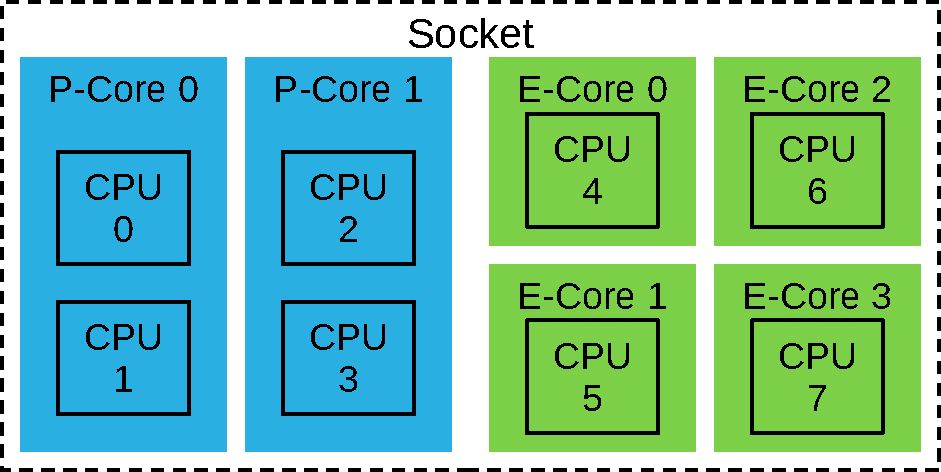
\includegraphics[width=0.65\linewidth]{images/heterogeneous_cpu_arch.pdf}
	\caption{Heterogeneous CPU architecture with two P-cores housing two hardware threads each and four E-cores with one CPU each on a single socket.}
	\label{fig:hetero-cpu-arch}
\end{figure}

For an operating system, this heterogeneity means that CPU time can no longer be treated as an interchangeable resource because the same workload can be completed in a different amount of time depending on which core type it is scheduled on.
This fact needs to be accounted for by any load-balancing policy targeting such hardware when trying to optimize for its given goal.

\subsection{Heterogeneous CPU Architecture}
\label{sec:hetero-cpu-arch}

Not only has the compute power of individual CPUs changed, but the physical placement of hardware threads has also moved from a uniform to a heterogeneous design.
Performance cores commonly combine multiple hardware threads onto a single physical core through SMT and share resources such as caches between them.
Efficiency cores typically retain a single hardware thread per core but are grouped into clusters that share a last-level cache among several cores (see Figure~\ref{fig:hetero-cpu-arch}).
One example of this architecture is the Intel Core i9-13900K Processor, \footnote{\href{https://www.intel.com/content/www/us/en/products/sku/230496/intel-core-i913900k-processor-36m-cache-up-to-5-80-ghz/specifications.html}{Intel Core i9-13900K Processor Specification}} used as testing hardware in this work.
This layout means that two hardware threads considered equally available by the operating system can in practice compete for the same shared cache, so a scheduler that is unaware of this topology risks placing threads in a way that looks balanced on paper but causes contention in hardware.

\cleardoublepage

%%% Local Variables:
%%% TeX-master: "diplom"
%%% End:

\chapter{Design}
\label{sec:design}

% Ist das zentrale Kapitel der Arbeit. Hier werden das Ziel sowie die
% eigenen Ideen, Wertungen, Entwurfsentscheidungen vorgebracht. Es kann
% sich lohnen, verschiedene Möglichkeiten durchzuspielen und dann
% explizit zu begründen, warum man sich für eine bestimmte entschieden
% hat. Dieses Kapitel sollte - zumindest in Stichworten - schon bei den
% ersten Festlegungen eines Entwurfs skizziert werden.
% Es wird sich aber in einer normal verlaufenden
% Arbeit dauernd etwas daran ändern. Das Kapitel darf nicht zu
% detailliert werden, sonst langweilt sich der Leser. Es ist sehr
% wichtig, das richtige Abstraktionsniveau zu finden. Beim Verfassen
% sollte man auf die Wiederverwendbarkeit des Textes achten.

% Plant man eine Veröffentlichung aus der Arbeit zu machen, können von
% diesem Kapitel Teile genommen werden. Das Kapitel wird in der Regel
% wohl mindestens 8 Seiten haben, mehr als 20 können ein Hinweis darauf
% sein, daß das Abstraktionsniveau verfehlt wurde.

This chapter presents the load balancing module that was designed throughout this theses.
It starts with an overview of the load balancer as a whole before exploring the individual components and their interactions.
Per component, multiple approaches are presented, and it is argued why a specific solution ended up in the final design.

\section{Architecture Overview}

The load balancing component consists of five main parts, four of which can be seen in Figure~\ref{fig:des:overview}.

\begin{figure}[h]
	\centering
	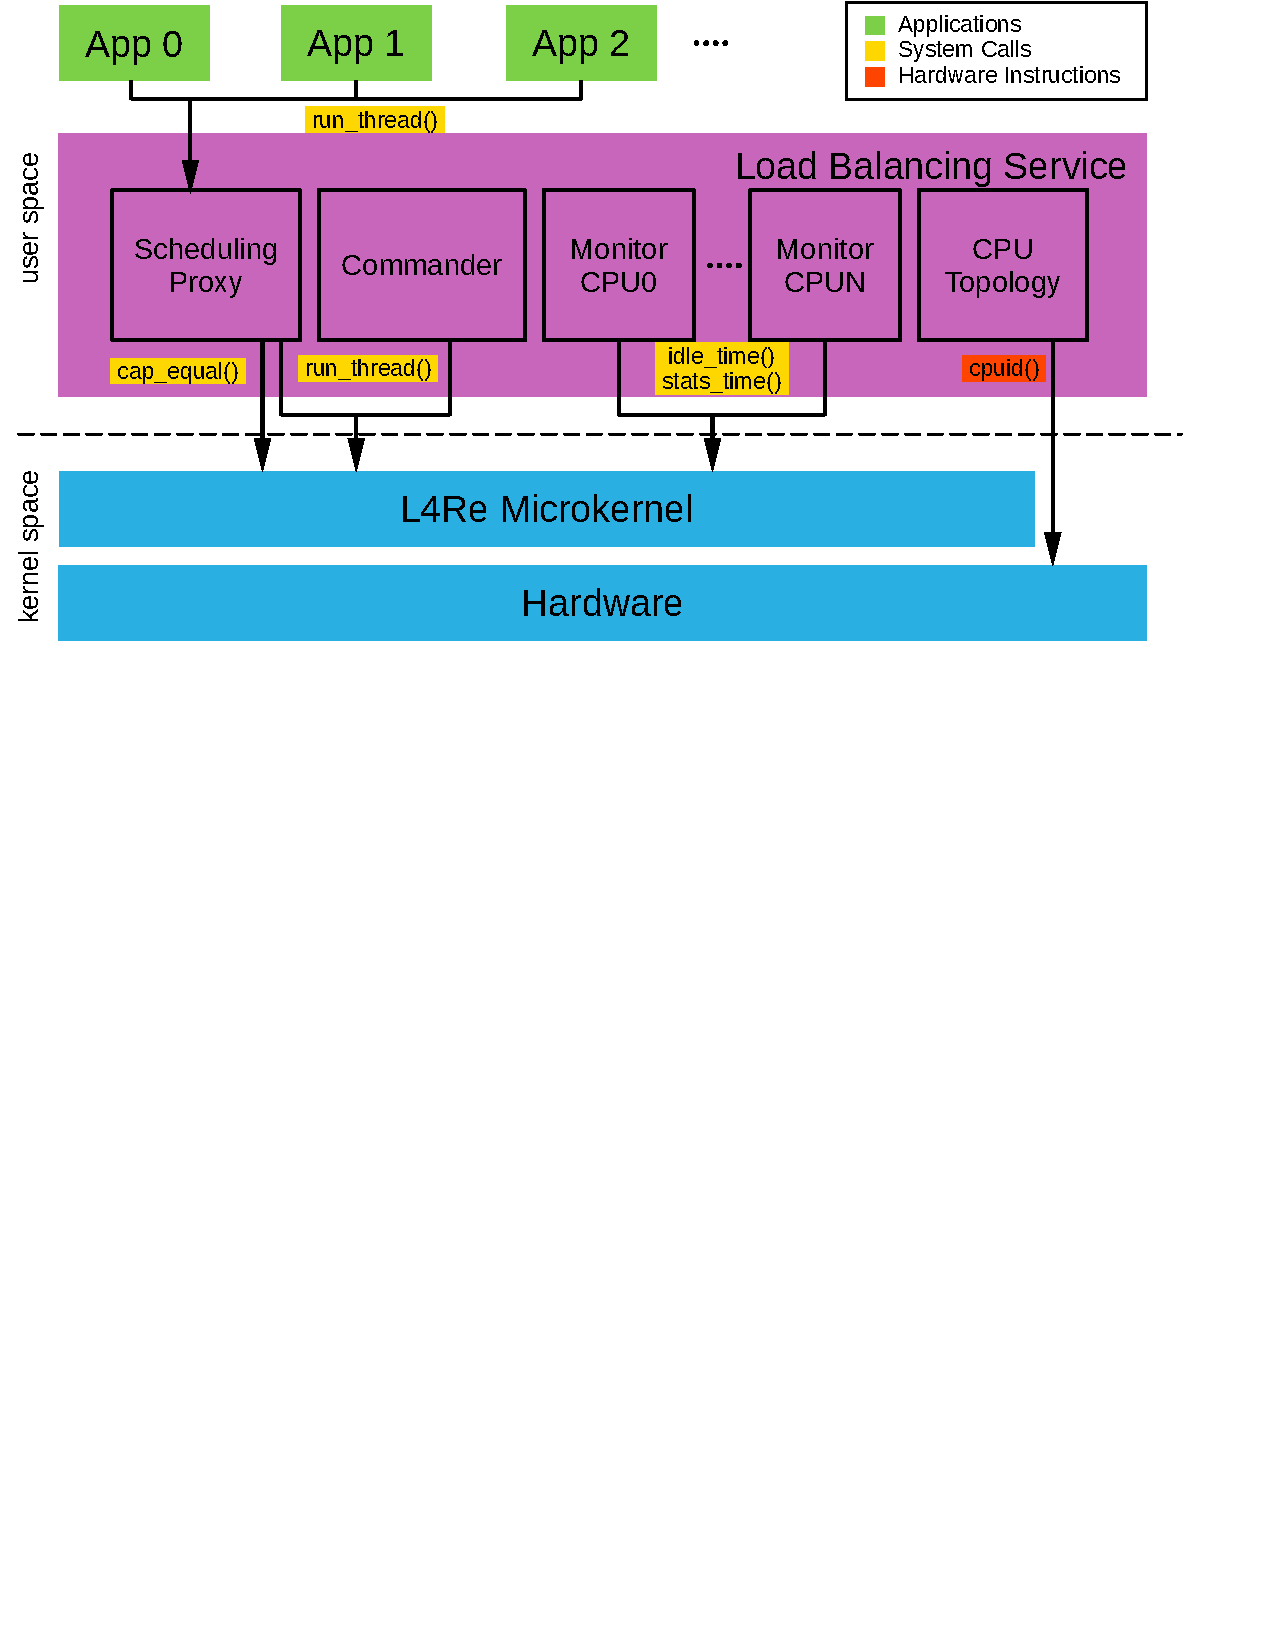
\includegraphics[trim={0 17.1cm 1.9cm 0}, clip, width=0.95\textwidth]{images/arch_overview_design.pdf}
	\caption{Architecture diagram at the design stage, showing the main components of the load balancing service and the communication between applications, the load balancer, and the kernel.}
	\label{fig:des:overview}
\end{figure}

The first component is a scheduling proxy that follows the L4Re proxy pattern (see Section~\ref{sec:proxy}) to receive scheduler calls like \texttt{run\_thread()} from the application to forward them to the actual kernel scheduler afterward.
During the interception, decisions can be made that enforce a given policy.

Second is the monitoring infrastructure consisting of one thread per CPU.
They track the runtime information of the idle thread and all regular scheduled threads on that CPU.

The commander is a thread that aggregates monitoring data and periodically triggers a rebalancing event.
During the rebalancing, overloaded and underloaded CPUs are identified, and migrations are ordered to bring the system back in balance.

Thread groups are the fourth and only component not visible in Figure~\ref{fig:des:overview}.
A thread group defines a CPU set that restricts members of that group to only run on dedicated CPUs allowed by the assigned CPU set.

The fifth component is the CPU topology, a structure that describes the topology of the hardware the load balancer observes.
In the case of non-uniform performance and structure of the CPUs, it retrieves information about processing speeds and location of hardware threads compared to cores, sockets, and further.

The whole design and implementation is based on the assumption that the underlying hardware architecture is x86.
Although the concepts would still suffice for other architectures, the concrete implementation would not work for individual components.

\section{Scheduling Proxy for Load Balancing}
\label{sec:des:proxy}

To appear as a scheduler instance, the load balancing proxy needs to implement all methods that the scheduler interface exposes.
The implemented functions can execute arbitrary policies as long as they adhere to the interface signature.
All calls of that interface except for \texttt{run\_thread} can be immediately forwarded to the scheduler of the scheduling proxy.
This does not necessarily need to be the kernel scheduler, as the proxy pattern allows layered scheduler instances on top of each other.

The entry point into the load balancing service is \texttt{run\_thread}.
This function is called by an application whenever it wants to run a specific thread with a set of scheduling parameters determining the thread's scheduling attributes.
It does not matter whether the thread is newly created or already exists.

The scheduling proxy shadows the threads and run queues currently in the system.
For this, it needs to compare the passed thread capability against all tracked capabilities to identify whether the thread is already being tracked.
If that is not be the case it is added to the bookkeeping structures.
Afterward, it will adapt all scheduling parameters according to its policy and forward the request to its designated scheduler.

\section{Monitoring the System State}
\label{sec:des:monitoring}

To make an informed migration decision, it is crucial to have information about the system state.
There are two system calls enabling this monitoring.
\begin{itemize}
	\item \texttt{L4::Scheduler::idle\_time()} is a call to the scheduler returning the total idle time of the CPU from which the request was made.
	\item \texttt{L4::Thread::stats\_time()} is taking a thread capability and returning the total runtime of the corresponding thread.
\end{itemize}
These methods allow identifying the load of a CPU and all threads currently tracked by the scheduling proxy.

A centralized approach checking every CPU and all threads of its run queue scales poorly with increasing CPU and thread counts; therefore, the design opts for a parallel approach.
For every CPU that was detected by the load balancer service, a designated monitoring thread (monitor) is spawned and pinned to this CPU.
It is responsible for periodically probing the idle thread's run time and state of the members of the local run queue.

Not only is it beneficial to have a run queue per CPU, but also the ready queue that only contains threads that are ready to run and, therefore, not blocked.
The scheduler interface does not provide a method like \texttt{get\_ready\_queue}.
This problem can be solved by extending the already existing \texttt{stats\_time()} call to not only return the runtime of the threads but also their thread state.
This call will be extended further in Section~\ref{sec:des:loba}.
Because the run queue needs to be iterated, it can be thereby annotated if a thread is currently ready or blocked.

\section{Commander Thread}
\label{sec:commander}

The commander thread (commander) is the central point of coordination for rebalancing decisions.
It collects all system information from the monitoring threads to make an informed migration decision.
This design falls into the category of centralized approaches for load balancing (see Section~\ref{sec:approaches}).
L4Re is built around the concept of strong isolation and the principle of least authority, or POLA for short.
Therefore, the system state information is distributed throughout multiple components that need to be collected separately, leading to a distributed system architecture.
Instead of having numerous instances access multiple sources at once, forcing complex behavior and access patterns, the design pivots to having one instance bundling multiple sources of information.
Three designs have been explored for aggregating monitoring information.

\subsection{Classic IPC.}

In L4Re, the IPC mechanism (see Section~\ref{sec:ipc}) is synchronous, so the commander would iterate through the monitoring threads.
This has the benefit of receiving up-to-date information from all CPUs and run queues.
However, the commander blocks for the whole time each monitor needs to retrieve the system state, resulting in poor scalability with growing CPU counts.
Additionally, the load balancer is a userland component, which means that every one of its threads can be preempted by other threads with higher priority.
This scenario is intended behavior, as a thread with higher priority should always be preferred by the system scheduler, but this could block the commander for an arbitrary amount of time when a monitor on a different CPU gets suspended.
At that point, the benefit of having up-to-date information from all CPUs does not hold anymore, as previously collected information will be outdated after blocking arbitrarily.

\subsection{Interrupt Notifications.}

To avoid iterating monitoring threads one after another but make use of having one monitor per CPU, the commander could be notified via interrupts.
Requesting the collection of all monitors at once and rebalancing when the final interrupt signals the return of the slowest monitor.
This approach parallelizes the monitoring process; hence, wall-clock time reduces from $\mathcal{O}(n)$ to $\mathcal{O}(1)$.
The drawback of this choice stems from most communication happening cross-CPU.
This assertion implies that for one request from the commander to a monitor and back, two IPIs are required (see Section~\ref{sec:cross-comm}), and excessive use of IPIs should be avoided at all costs.
Further, the problem of preempted monitors needs to be handled, for example, by bounding the waiting time of the commander with a timeout.
At that point this solution is more complex and costly than the previous approach.

\subsection{Asynchronous and Non-Blocking Coordination via Absolute Timeouts.}
\label{sec:abs-timeouts}

L4Re provides a primitive that allows a thread to not only sleep for a relative amount of time but also until an absolute system time is reached.
This mechanism allows the monitors and the commander to sleep until the next monitoring interval is reached.
The monitoring threads wake up first and retrieve the system state, and the commander sleeps for a fraction of the monitoring interval longer.
Upon waking up, it needs to be checked via timestamps to see if the monitors were able to update the system state in time to not read outdated information.
This approach combines the benefits of both previous solutions because an absolute timeout is implemented using efficient core-local IPC while also retaining the parallelism in monitoring.
This solution assumes a synchronized system clock for all participants, which is provided by the L4Re microkernel.

\paragraph{Key Insight.}
\label{sec:insight-prio}

The problem of load balancing threads getting preempted leads to an important discovery.
The load balancer cannot properly balance tracked threads that have a higher priority than the priority it is scheduled on itself.
This results from designing a scheduling component in userland, as the code does not run in kernel mode and is not only interruptible but also preemptible.
Therefore, the load balancer should obtain the highest priority possible, so the worst case would be round-robin scheduling with other threads of the same (maximum) priority.

\section{Load Balancing}
\label{sec:des:loba}

To be able to balance workload inside the system, a definition of load and, further, of over- and underload needs to be determined.
The intuitive solution would be to work with the current CPU utilization (from now on referred to as CPU load), which can be determined by the runtime of the CPU's idle thread.
This approach works well until the CPUs reach a load of 100\,\% or, inversely, an idle time of 0.
If ready threads start to accumulate faster on a CPU than they can be served, it is desirable to treat all threads fairly and move them to other CPUs that may also be at 100\% capacity but with shorter ready queues.

Thus, using CPU load as a one-dimensional balancing metric is insufficient to solve a multidimensional problem.
The USE (utilization, saturation, and errors) method, proposed by Brendan Gregg~\cite{use_method_gregg}, identifies utilization as just one dimension of performance.
Saturation needs to be regarded as well for CPU workloads, as it describes the pressure that accumulates on a CPU by growing run queue sizes.
Errors can be ignored in the scope of this work because USE was introduced in the context of distributed network systems, and CPUs do not drop instructions.

Linux employs a virtual runtime (see Section~\ref{sec:best-effort}) to capture utilization and saturation at once.
This method cannot be used to define CPU load either because L4Re is based on priorities and does not use time budgets for threads.

The metric used in this work builds upon the information of whether a thread was preempted during its time slice or gave up the CPU voluntarily.
Preemptions can happen either through a thread of higher priority becoming ready and replacing the previously running thread or the timer interrupt at the end of the time slice.  
Voluntarily yielding the CPU is considered everything that is not covered by preemption, for example, calling \texttt{yield()}, making an IPC call, or blocking through sleeping.
Capturing this information for every thread gives insight into how compute-demanding it was during its previous time slices.
Accumulating this metric for the whole run queue of a CPU strongly correlates with the CPU time consumed, but it also can outgrow 100\% CPU load.
This characteristic is important because threads that were compute-heavy in the past and are now suspended still add pressure to that CPU, although they do not receive any CPU time.
Of course, this metric can be tricked under special circumstances when threads would use a large amount of their time slice and then yield the CPU to seem computationally lightweight.
This behavior is a potential problem but not assumed as the average case.
Hence, the metric is able to capture utilization and saturation, making it more robust than just pure CPU load.
The metric derived from the tracked preemptions and used to determine the load of a CPU is called virtual load or \texttt{vload}.

The preemptions of a thread need to be collected for every thread tracked in the system.
This can again be solved by extending the already existing \texttt{stats\_time()} system call to additionally return the preemptions of a thread in addition to its blocked or ready state and its used CPU time.

\section{Thread Groups}
\label{sec:thread-groups}

Thread groups were created to solve the task of providing explicit scheduling groups for threads inside the system.
One example of a component that assumes separation of threads is the L4Re virtual machine monitor, UVMM.
When it creates multiple vCPUs, it is desirable to have them running on different physical CPUs.
Mostly because timesharing for vCPUs of the same VM does not make any sense, and busy-waiting primitives are used in virtual machines.
In addition to having vCPUs separated on hardware at all times, they are implemented as multiple threads.
The threads that make up one vCPU need to be placed on the same physical CPU at all times.

To employ a single source of truth, thread groups were introduced.
One unique group can be created per CPU scheduling set containing all the threads that were issued with the corresponding group's CPU set.
The member threads in a group are only allowed to run on the CPUs specified by the group's CPU set.
The layout of CPU sets is not restricted to any particular subset structure, so the number of possible thread groups is $2^n$ for $n$ available physical CPUs.
In practice, only a small subset of groups is used.
Additionally, the L4Re data type specifying a CPU set (\texttt{l4\_sched\_cpu\_set\_t}) does not allow all possible cases.

\begin{figure}[h]
	\centering
	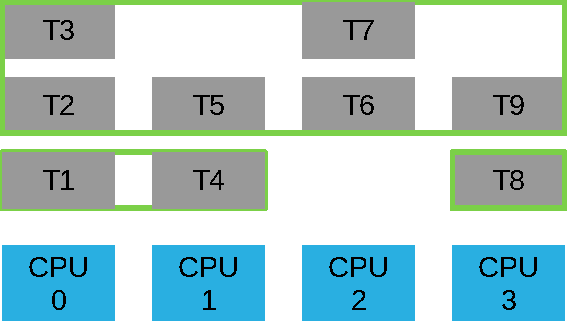
\includegraphics[width=0.6\textwidth]{images/thread_groups.pdf}
	\caption{Thread group example with four CPUs, nine threads (T), and three thread groups (green frames) limiting the placement of their threads to the CPUs they span. Thread group \{T1, T4\} on CPU0 and CPU1, group \{T2, T3, T5, T6, T7, T9\} on all CPUs, and group \{T8\} on CPU3.}
	\label{fig:thread-groups}
\end{figure}

If individual groups would experience poor performance, there is the option to reassign the physical CPUs that represent the available CPU sets to the groups.
The constraint that certain groups are not allowed to share physical CPUs during the reordering must not be violated.
Therefore, groups do not share physical CPUs with other groups; they are disjoint from in the originally assigned CPU set, and this remains true during reassignment as well.

The moment groups would have their CPU sets reassigned, applications that rely on thread pinning could have that assumption violated.
A countermeasure to this problem is the introduction of thread groups that represent pinned threads and do not have their CPU set reassigned.
This posed the problem of receiving the information if a thread should be pinned or not via the \texttt{run\_thread()} call.
One option would be to add a field to the scheduling parameters that are passed during the call.
In doing so, one would create severe ripple effects throughout the whole L4Re framework, as either a new scheduling parameter type would need to be created or all existing instances would require adaptation.
The approach chosen for this work was to add another \texttt{run\_thread\_pinned()} call to the scheduler interface, which passes a parameter if the thread should be pinned or not.

\section{Priority Translation}

The placement decision made during the handling of \texttt{run\_thread()} is just one policy enforced by the proxy; another can be to alternate the scheduling priority of a thread.
A scheduling proxy can be used to restrict or broaden the available priority band in any way.
Hence, the load balancer has the ability to move applications to low-priority, best-effort, or high-priority, real-time execution.
During the creation of the load balancer, a priority band can be assigned that then is used by the proxy to have threads end up only inside the specified priorities.

In the scope of this work two policies for priority translation were implemented from which a user can choose from during the creation of the load balancer.
When no strategy is specified, the default policy is chosen.

\paragraph{Cutoff.}

The default strategy is a cutoff applied to the resulting priority band.
If a thread is issued with a priority lower than the minimum, it is raised to the minimum.
Vice versa, the priority is lowered if the thread is issued with a priority higher than the maximum.
When the issued priority is inside the allowed priority band, no modification is made.

\paragraph{Priority Scaling.}

The second strategy scales the priority from the system's default priority band (0-255) to the specified range.
The relative position of the issued priority stays the same compared to the boundaries of the destination priority range. This preserves the relative priority differences within an application.

\medskip

Although both strategies may prove disadvantageous depending on the specific use case, the design allows for easy extension with additional policies tailored to future requirements.
Priority translation was not the focus of this thesis, so the two implemented strategies should be regarded as a default implementation rather than a central contribution.

\paragraph{Key Insight.}

L4Re defines its scheduling priorities as core-local.
This concept no longer holds the moment a thread needs to be migrated from one CPU to another.
Beforehand, a migration could only be issued by an application, which then needed to pass corresponding scheduling parameters with a given priority to the scheduler.
Therefore, the decision of what priority to advance with was left to the user.
To solve the problem of core-local priorities, they are assumed to be global for the load balancing component.

\section{CPU Topology}

The reading of the CPU topology is the main reason why this work relies on the x86 architecture, because it provides the \texttt{cpuid()} assembly instruction in userland.
Architectures such as ARM do not expose an equivalent instruction outside the kernel.
Retrieving the same topology information there would require extending the kernel itself and adding an interface through which userland could query the collected data, since userland has no direct means of reading it on its own.
\texttt{cpuid()} allows reading CPU-specific hardware information such as vendor identification, processor signature, feature flags, cache and TLB details, as well as power and thermal information~\cite{intel-cpuid}.
Tools like \texttt{lstopo} make use of most of this data to gain full insight into the hardware on which the operating system is executed.
For this work, the topology information alone is sufficient.

The design for reading CPU information is heavily inspired by an internal, non-public, existing L4Re userland module.
It reads the CPU topology to manage the separation of CPUs for applications that prohibit core sharing.
Because caches can be shared between multiple CPUs on the same physical core, a malicious thread could otherwise read cache information belonging to another application running on a CPU sharing that core.
To eliminate this threat, potentially affected applications require their threads to run on cores that are isolated and shared with no other application.

Evaluating the CPU information was simplified by reading all CPUs first and constructing the topology once afterward, rather than exploring a CPU and constructing part of the topology before reading the next one.

\subsection{CPU Performance Detection}
\label{sec:cpu-performance}

Not only is it beneficial to have insight into the CPU topology when hardware is asymmetric (see Section~\ref{sec:hetero-cpu-arch}), but also it is advantageous if the CPUs themselves are heterogeneous.
Distinguishing performance and efficiency cores is crucial, as they will behave differently under the same workload.

For the design in this work, an idea from the paper of Li and colleagues~\cite{faster-core-first} was adopted, where load balancing is made AMP-aware by scaling the compute power of each CPU based on its instructions executed per cycle.
By doing so, it breaks the heterogeneous hardware down to uniform processing, as the load of each CPU can be scaled by its processing speed.
Scaling CPU performance to obtain a uniform hardware abstraction works against the idea of having asymmetric CPUs in the first place, but this shows that not only is multiprocessor scheduling a non-trivial problem to solve, but it also gets even harder when underlying hardware is non-uniform.

The detection is done via microbenchmarks during the start phase of the load balancer.
For this one thread is spawned to each CPU measuring processing speed next to reading the CPU topology via \texttt{cpuid()}.
The compute performance of each CPU is then compared and scaled upwards relative to the slowest result.
The performance value is scaled in steps of 0.1.
Hence, a CPU scaled with 3.5 is three and a half times faster than the slowest CPU in the system.
To avoid unnecessary computation, the performance measurements are not done when the topology information returns that the system is uniform and therefore not composed of performance and efficiency cores.

Performance and efficiency cores are powerful in theory, but it is difficult to fully harness them as an operating system in practice.
Doing so requires sophisticated monitoring of the threads' behavior to classify them correctly, which is even more difficult in a microkernel and thus out of scope for this thesis.
Established operating systems like macOS, Windows, or Linux can make use of this kind of hardware because they can analyze their threads' behavior thoroughly.

\cleardoublepage

%%% Local Variables:
%%% TeX-master: "diplom"
%%% End:

\chapter{Implementation}
\label{sec:implementation}

% Hier greift man einige wenige, interessante Gesichtspunkte der
% Implementierung heraus. Das Kapitel darf nicht mit Dokumentation oder
% gar Programmkommentaren verwechselt werden. Es kann vorkommen, daß
% sehr viele Gesichtspunkte aufgegriffen werden müssen, ist aber nicht
% sehr häufig. Zweck dieses Kapitels ist einerseits, glaubhaft zu
% machen, daß man es bei der Arbeit nicht mit einem "Papiertiger"
% sondern einem real existierenden System zu tun hat. Es ist sicherlich
% auch ein sehr wichtiger Text für jemanden, der die Arbeit später
% fortsetzt. Der dritte Gesichtspunkt dabei ist, einem Leser einen etwas
% tieferen Einblick in die Technik zu geben, mit der man sich hier
% beschäftigt. Schöne Bespiele sind "War Stories", also Dinge mit denen
% man besonders zu kämpfen hatte, oder eine konkrete, beispielhafte
% Verfeinerung einer der in Kapitel 3 vorgestellten Ideen. Auch hier
% gilt, mehr als 20 Seiten liest keiner, aber das ist hierbei nicht so
% schlimm, weil man die Lektüre ja einfach abbrechen kann, ohne den
% Faden zu verlieren. Vollständige Quellprogramme haben in einer Arbeit
% nichts zu suchen, auch nicht im Anhang, sondern gehören auf Rechner,
% auf denen man sie sich ansehen kann.

In this chapter implementation details will be discussed.
It elaborates on the hurdles that were encountered during the development of the load balancer and how they were overcome.
Most of the problems discussed root in the design of a microkernel-based operating system, which is comparable to a distributed system, and the scheduler, which is often designed to be part of the kernel, is now implemented in user space.

\section{Scheduling Proxy}
\label{sec:impl:proxy}

The scheduling proxy handles all functionality that is exposed by the scheduler interface but mainly \texttt{run\_thread()}.
Because the function itself is straightforward, only the most interesting details are investigated further in the following section.
The proxy is the entity in the load balancer that maintains the addition of new threads into the bookkeeping structures and, therefore, their capabilities.
They are one of the main security features L4Re is built upon and require special handling.

\subsection{Capability Slots}
\label{sec:impl:cap-slots}

Capabilities are the primitive to control access rights to objects in L4Re.
To prevent applications from maliciously manipulating their own domain of access, capabilities are managed by the application but maintained in kernel space by the kernel.
The app only has access to a so-called capability table that allows the invocation of entries to request the kernel to execute an operation with the object behind the specified capability.
Thus, the userland only operates on capability table slots, as can be seen in Figure~\ref{fig:cap-table}.

\begin{figure}[h]
	\centering
	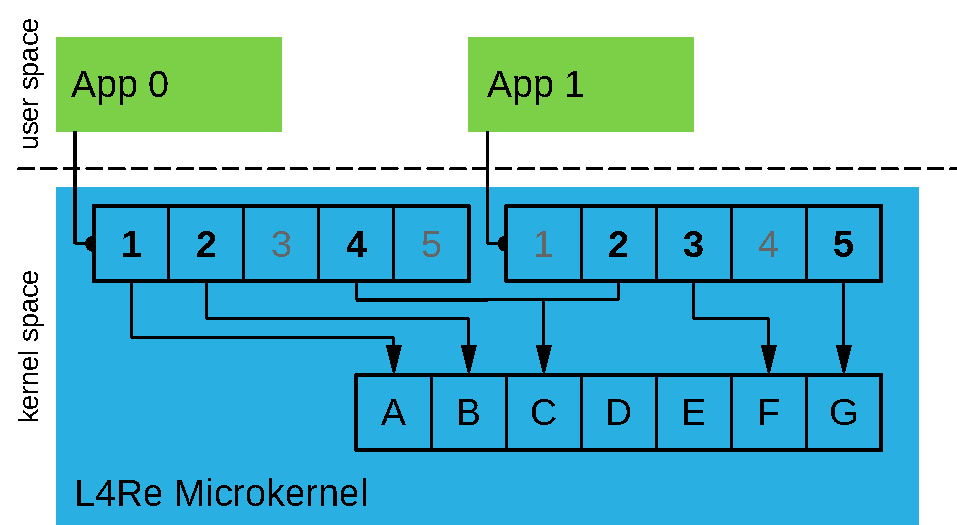
\includegraphics[width=0.7\linewidth]{images/capability_table.pdf}
	\caption{L4Re capability tables and entries (indices) of applications referencing kernel objects (characters) in kernel space.}
	\label{fig:cap-table}
\end{figure}

The moment the scheduling proxy receives a new thread capability via \texttt{run\_thread()}, it needs to check if it already tracks that thread.
The proxy does not have access to the actual capability objects but can only request the kernel to act upon a given index of the capability table.
This table has a receive slot (index) that determines where the next incoming capability is written to.
The moment the scheduling proxy decides to add a thread into its bookkeeping, it takes ownership of the thread's capability.
When doing so, the receive slot must be moved to a new unoccupied table index; otherwise, the next call of \texttt{run\_thread()} will overwrite the previously stored capability.
An overwritten capability would thus lead to threads the proxy took ownership of but cannot access anymore, making it unable to migrate them in the future.
To solve this leakage of dangling threads, the proxy needs to call \texttt{realloc\_rcv\_cap()} after taking ownership of an incoming capability.
This moves the table entry to an empty slot where new capabilities can be received.
Because memory is finite, the capability table is limited in size, and \texttt{realloc\_rcv\_cap()} will return an error when it runs out of empty capability slots.
This error indicates that the table is fully occupied and the load balancer is not capable of handling any more new threads because no empty slot is left in the table.
This scenario does not present a practical limitation, as the table size can be increased up to thousands or millions of entries.

\subsection{Access Rights}

The scheduling proxy only acts upon indices in the table instead of capabilities themselves, which means that it is not able to determine if the capabilities stored in two slots point to the same object.
The L4Re microkernel provides a system call to determine if two capabilities are equal called \texttt{cap\_equal()}.
It compares the capabilities stored in the specified table entries and returns a boolean value.
This mechanism allows the scheduling proxy to check if the received capability by \texttt{run\_thread()} is unique or already tracked.
The first problem exposed by this approach is that identifying a thread requires $n$ system calls when $n$ threads are already tracked, just to compare capabilities.
This solution could be improved by batching the requests to the kernel; however, Section~\ref{sec:overhead-analysis} will show that the overhead of the scheduling proxy can be ignored and does not pose a scalability problem.
The second, much more serious problem that results in erroneous behavior if not handled correctly is that capabilities are the union of an object pointer and the assigned rights to that object.
Two capabilities referencing the same thread but with different access rights are not considered equal.
This poses a problem for the load balancer because applications can call \texttt{run\_thread} on the same thread multiple times.
The \texttt{pthread} library used to create threads invokes \texttt{run\_thread} with a reduced set of access rights.
Although the design of \texttt{cap\_equal()} is absolutely correct, this behavior will break the bookkeeping structures of the load balancer.

To avoid this all at once, the kernel was extended by the \texttt{cap\_equal\_no\_rights()} system call.
It still compares two capabilities for equality but does not regard the associated access rights as only object references.
This way, the scheduling proxy can rely on the assumption that a capability to a thread is unique whenever it points to the same thread.

\section{Monitoring}
\label{sec:monitoring}

\subsection{Dead Threads}

In Section~\ref{sec:des:proxy}, it was discussed that the scheduling proxy represents the entry point of a tracked thread into the load balancer because it is registered there.
The problem with implementing a scheduling proxy in userland is that it is not not notified when a tracked thread exits the system.
Instead of registering the proxy to be notified by the kernel with an interrupt whenever there is a dead thread in its domain, it is easier and more efficient to extend a mechanism already in use.
The \texttt{stats\_time()} system call needs to be invoked for every tracked thread each monitoring interval (see Section~\ref{sec:des:monitoring}).
An invocation with the capability of a thread that has already left the system results in an IPC error message.
This signals to the monitoring thread that it can now delete the affected thread from the bookkeeping structures of the load balancer.

The deletion of a dead thread needs to be managed properly to avoid corrupting the bookkeeping because there are multiple tracking data structures referencing threads.
Tracked threads reside in their appropriate run queue and thread group, defining the allowed CPU scheduling set (see Section~\ref{sec:thread-groups}).
Because the monitoring infrastructure uses run queues to iterate through threads for probing, they have been made the governing data structure.
A dead thread is deleted from its run queue, and the destructor removes the thread through back references from its assigned scheduling group.
If a thread group runs empty the moment a thread deregisters from it, the group triggers its own removal from the set of groups.

\subsection{Thread Probing}
\label{sec:probing}

Monitoring threads iterate all threads contained in the shadow run queue assigned to the CPU they are running on (see Section~\ref{sec:des:monitoring}).
Migrations are not instant, and thus there will be a point in time where a thread is still in migration transition, but the load balancer has already moved the tracked instance to its destination run queue in its bookkeeping.
This leads to complications when the migration is not finished until the next monitoring cycle, as a monitor will try to probe a thread that is not on its CPU yet.
When issuing the system call, the kernel will either look up the information needed right away when the requested thread is on the same CPU as the caller, or it will start a DRQ (see Section~\ref{sec:cross-comm}) on behalf of the caller to the requested thread.
This behavior poses a problem to the monitor because if a thread is still in migration transition, the probing request will not be executed with the priority of the monitor anymore but with the priority of the requested thread.
In most cases, this will lead to a scenario that is known as \enquote{priority inversion.}
The monitor with a high priority blocks on a low priority thread, which is then preempted by a medium priority thread on the destination CPU.
Inevitably inverting the priority of the monitor because it is delayed by the medium-priority thread for an arbitrary amount of time despite having higher priority~\cite{priority-inheritance-protocols}.
Further, system calls cannot be requested using timeouts; therefore, the monitor would be stuck until the requested thread handled the DRQ.
To avoid this interaction, the \texttt{stats\_time()} system call was modified to return an error code instead of executing a DRQ.
It comes at the cost of working with outdated information for that tracked thread and monitoring cycle but assures that the load balancer infrastructure cannot block during system calls.

\subsection{Timing}

Numerous components of the load balancer require precise and synchronized timing to function correctly.
The commander and monitors use absolute timeouts to orchestrate themselves (see Section~\ref{sec:abs-timeouts}).
The proxy and commander use precise timing to identify monitors whose information is outdated, and the monitoring threads themselves rely on it because of the CPU idle time and thread probing.
To provide exact timing to the load balancer, the L4Re microkernel needs to support \texttt{FINE\_GRAINED\_CPUTIME}.
When enabled, the kernel then calculates the exact CPU usage of a thread on every context switch instead of \si{\ms} granularity.
Additionally, the \texttt{SYNC\_CLOCK} option should to be set, which requires \texttt{HAS\_SYNC\_CLOCK} to ensure that all CPUs can read the same system time.
It has to be mentioned that \texttt{SYNC\_CLOCK} could lead to complications when operating on processors that have more than one hardware socket.
Without both features activated, the time received by the \texttt{idle\_time()} system call and the value returned by \texttt{l4\_kip\_clock(l4\_kip())} deviated heavily, leading to incorrect results when calculating the CPU load from idle and passed time.

\iffalse
% This is a debatable topic and should not be used
\section{Priority Usage}

Section~\ref{sec:insight-prio} discusses the idea that the load balancer threads should assign themselves the highest priority possible.
In the default priority band, this would translate to 255, which is a reserved priority for important tasks only.
The only instances with that priority are the root task Moe, the pager, and the interrupt handler of each application ITAS and software interrupt requests (SW IRQs).
The one monitor per CPU, the scheduling proxy on CPU1, and the commander on either CPU1 or CPU2 would then compete against Moe and ITAS in round-robin scheduling or during message delivery of IPC communication with SW IRQs at the same receiver.
Interrupt delivery and its handling are assumed to be as fast as possible to reduce interrupt latency.
In a priority-based operating system, this principle is followed through as well, but the thread with the highest priority gets to monopolize the CPU anyway.
Hence, even if the software IRQ is delivered and handled with the highest importance, an application with a lower priority than the load balancer will be suspended when monitoring or rebalancing is taking place.
Therefore, it does not matter to the application if the load balancer is competing with those or not because it will be preempted nevertheless.
Further, SW IRQs would only compete with IPC messages of the load balancer if they had the same destination, but all load balancer components have self-contained communication, meaning they only exchange IPC with themselves or make system calls.
Hence, they would not interfere with SW IRQs in the first place, leading to the decision that a priority of 255 is safe to use for the load balancing components.

Although not a disturbance within the scope of this work, it should be investigated and discussed for future systems if the load balancer's importance requires it to use priority 255 or if 254 would be sufficient as well.
This would make it inferior to Moe on CPU0 but would adhere to the guideline of having the maximum priority reserved.

\fi

\section{Load Balancing}
\label{sec:impl:loba}

\subsection{Tracking Preemptions}

In Section~\ref{sec:des:loba}, the metric \texttt{vload} was introduced, allowing for robust CPU monitoring.
The preemptions, the thread's demand, and ultimately the virtual load metric are tracked using a sliding window approach.
For this an array structure is needed that captures the previous $n$ preemptions or yields of the thread.	
The information is provided by the kernel, and therefore it needs to track such an array for every thread in the system.
It is preferred to solve this problem with a stateless and memory-efficient approach.
An actual array paired with a pointer to create a looping ring buffer would be a viable implementation for the job but is way too complex for the actual task.
Ultimately, the sliding window needs to store zeros and ones, which can be done much more space- and time-efficiently by a single machine word.
When the timer tick hits or the thread yields, the kernel can simply shift the machine word left once and add the new decision at the least significant bit.
In doing so, this gets rid of an actual array, which would also be more difficult to transfer via the system call than a single register is.

\subsection{Calculating Demand}

Every bit of the preemption machine word adds to a demand value.
The older a bit is in time, the lower its added value is.
This concept assumes that information further in the past has less correlation with what will happen in the future.
For determining the half-life of the preemption bits, the Linux scheduler was considered.
It uses aging when calculating its virtual runtime, and information that is \SI{32}{\ms} in the past only accounts for half its original weight.

Hence, the demand is calculated using the sum of a geometric sequence.
\[
S_n = x_1 y^1 + x_2 y^2 + x_3 y^3 + \dots + x_n y^n = \sum_{k=1}^{n} x_k y^k
\]
Using a machine word also comes in handy when calculating this sum.
Instead of iterating an array, the machine word can be used as the condition of a while loop, shifting the register each iteration; therefore, the loop ends when the machine word is all zeros, sparing unnecessary iterations.
Further, the half-life of \SI{32}{\ms} makes the final bits of no influence, as their contribution is marginal.
This allows for masking the preemption machine word beforehand to only be left with significant bits and exiting the while loop early after necessary parts were computed.

\subsection{Rebalancing}
\label{sec:rebalancing}

Load balancing is kept simple by calculating the average vload over all CPUs and then determining an upper and lower bound by adding or subtracting 20\,\% from the average.
Thereby, the \texttt{vload} of a CPU is the sum of the \texttt{vload} of its run queue threads divided by the performance factor of this CPU.
All CPUs above the calculated upper bound and at 90\% actual CPU load are considered overloaded, and all below the lower bound are underloaded.
If an overloaded CPU only has one thread in its run queue, it is skipped, except for CPU0, as the L4Re infrastructure threads like Moe are placed there.
Per overloaded source CPU, one thread will be moved to an underloaded destination CPU.
This decision is made using a scoring function that considers the destination's load, the thread's \texttt{vload} and migration cost, and the destination's capacity for the thread's priority (1 minus the CPU usage of threads of higher or equal priority).
The cost of a migration is estimated by using the CPU time a thread consumed during the previous monitoring interval, as it is assumed that a high CPU usage correlates with caches still being warm. 
This metric is taken into account because it is expensive to reload cache content at the destination CPU.
A migration of a thread that would overload the destination is disregarded.
Also the \texttt{vload} of every planned migration is projected onto the \texttt{vload} of the destination CPU to prevent pile up on a CPU that seems favorable.
The migrations with the best scores are stored and executed after the rebalancing algorithm is done.

\paragraph{Key Insight.}
\label{sec:insight-placement}

There will be a hidden load the load balancer cannot measure because it is caused by threads that are not tracked by its bookkeeping, including the load balancer itself.
The most common example for this phenomenon is Moe because it is needed to launch a load balancer instance and can therefore not use it as its scheduler.
It is always located on CPU0 and activates occasionally when system-level background tasks need to be done, like allocating or freeing memory; thus, it does not constantly cause load but rather does so in bursts. 
This behavior is the reason why the scheduler proxy is moved to CPU1 and the commander to CPU2 (if available) so they do not get interrupted by those occasional spikes in hidden CPU time consumption.

\section{Thread Groups}

It is crucial to provide mutually exclusive CPU sets to vCPUs when their thread groups receive a reassignment of allowed physical CPUs (see Section~\ref{sec:thread-groups}).
This separation is the reason why every group needs to track all other groups it is disjunctive with.
When constructing a new CPU assignment, all those tracked groups need to be regarded to assure that vCPUs do not end up on the same physical CPU.
The problem is a simpler version of the bin packing problem and can therefore be efficiently shortcut~\cite{binpacking}.
The approach of this work uses the \texttt{std::bitset<N>} struct from the standard library, with N being the maximal number of CPUs the load balancer is able to detect.
It is used to represent the CPU set as a bitmap, where each bit corresponds to exactly one physical CPU.
The bitset is a data structure whose size is known at compile time, making it fast, as boolean operators are supported.

Calculating the new CPU assignment requires a bitset with all physically available CPUs.
It is stripped of all bits that are set in disjunctive groups' bitsets, leaving all available CPUs from which the group can now choose.
The calculation can be done efficiently by applying a bitwise \texttt{AND} on the available and inverse disjunctive bitsets iteratively.
The affected group can then select CPUs from this available set until its own CPU demand is satisfied, or in other words, until the population count of the assigned set is equal to the population count of the original CPU set.
The selection process can implement any policy.
For this work the CPUs with the lowest \texttt{vload} are chosen first.
The calculation and assignment process is then carried through for all groups in ascending order of the population count of the originally assigned CPU sets.

\section{Thread Safety}

The load balancer is designed as a multithreaded application working on shared data structures.
When resources are operated using multiple threads, their write accesses need to be mutually exclusive to avoid corrupting the state of the data structure.
The most common primitive operating system provides for locking with a mutex (lock).
The thread that currently holds the mutex can therefore safely read and modify structures like the thread groups and run queues while other threads trying to acquire the lock are blocked.
For reading and writing simple state structures such as tracked threads or CPU states, this would introduce unnecessary overhead without yielding any benefits compared to using atomic operations provided by all architectures.
Only when the size of the attribute that needs to be protected disallows the use of atomics, a mutex is again used to make that attribute thread safe.
The two mechanisms of atomic operations and mutex locking allow for concurrent access of the shared structures.

\section{Distributed System in Userland}
\label{sec:distributed-system}

Section~\ref{sec:commander} states that the design of the load balancing component on top of the L4Re microkernel-based architecture leads to a distributed system.
The scheduling proxy, commander, and all monitors can be preempted at any time.
Therefore, they require an implementation that does not halt the entire load balancer just because one thread of the monitoring infrastructure was preempted.
The load balancer is designed to orchestrate threads on multiple CPUs; hence, it also needs to scale well with a rising number of physical cores.
This challenge can be taken on with an asynchronous approach.

The only threads issuing migrations and, therefore, making decisions are the scheduling proxy and commander.
If either one should be preempted, that is simply user-space load balancing, which is undesirable but unavoidable.
What should be avoided is that a monitoring thread blocks either the proxy or the commander, making them unable to make an informed placement decision.
This scenario can happen because of the introduction of thread-safe accesses and locks.
When a monitor is suspended while iterating its CPU's run queue, it still holds the run queue's mutex.
If the commander or proxy then tries to insert a thread into that run queue, they will block because they need to acquire the mutex first.
If all load balancer components are run with the highest system priority, the blocking is bounded, as on the same priority round-robin scheduling is employed, but if this happens with a lower priority, the suspension could be arbitrary.

It is not possible to eliminate this problem entirely without the use of lock- or wait-free implementations.
They usually have a good worst-case but slow average-case performance.
The approach in this thesis (see Section~\ref{sec:abs-timeouts}) makes use of mutex primitives and is therefore prone to special cases of blocking that could lead to scenarios described previously.
The monitors are iterating their assigned run queue to probe all threads on their CPU.
This could lead to the commander being blocked.
The monitor also writes information about the CPU state that includes a timestamp of the update.
Writing the timestamp is the final operation a monitoring thread does in its monitoring cycle before blocking itself with an absolute timeout.
Therefore, the commander can first check the timestamps of all CPU states and verify if their information is outdated.
Once such a state is detected, it is marked by the commander setting its \texttt{vload} to the maximum possible value the attribute can hold.
The commander will proceed rebalancing with all those CPUs that are considered in time.
The same checking mechanism is employed by the scheduling proxy.
However, the scheduling proxy is required to proceed with all CPUs because of thread pinning.
When threads request to be pinned to a specific CPU, the proxy needs to be able to migrate them to that CPU even if it is currently not favorable.

\subsection{Consistent \texttt{vload} Views Through Write Ordering}
\label{sec:vload-updates}

During the development, a centralized and parallel approach has been implemented to update the \text{vload} of the CPU states.
The whole load balancer is implemented and benchmarked with the centralized solution.
The parallel solution was only measured regarding overhead.
During the writing of the thesis, it was determined that the parallel approach does not raise any complications with regard to the multithreaded access pattern.

\paragraph{Centralized.}

In the centralized implementation, the commander iterates all synchronized CPUs to update their \texttt{vload}.
Doing so, it iterates the run queue of every CPU, which would be potentially blocking if unsynchronized CPUs were iterated as well.
As they have been marked beforehand, this does not pose a threat of blocking directly.
There are scenarios that could lead to the commander being blocked by a monitor, but they would need to be constructed carefully and are therefore not regarded as the average case.

The chain of thought for this approach was that proxy and commander need to detect and mark outdated information of CPUs to reduce the chance of blocking.
A marked CPU gets its \texttt{vload} value set to \texttt{UINT64\_MAX} to make it unfavorable for any further selection process.
If the calculation of the CPU's virtual load were carried out by the monitors, they could overwrite this value at arbitrary points in time, also during the rebalancing and the time the proxy picks a CPU on which a thread should run.

The overwrite does not raise any problem with the rebalancing, as the commander only proceeds with synchronized CPUs.
Already marked CPUs could therefore be overwritten without any effect, as their \texttt{vload} is not read until the next monitoring loop.
The scheduling proxy, on the other hand, is not allowed to make any CPU restrictions.
If a thread needs to be pinned, the proxy has to be able to choose from all CPUs, even those that are currently blocked because pinning is a hard constraint.

\paragraph{Parallel.}

The \texttt{vload} can also be updated by the monitors during their probing cycle.
This has the potential to yield a speedup equivalent to the number of CPUs in the system because it eliminates the single commander instance as a bottleneck.
Theoretically, a parallel approach scales better than the centralized counterpart.
The previously stated concern of arbitrary overwrites while the scheduling proxy has to pick a CPU is also unfounded.
All accesses to the \texttt{vload} value of a CPU state are done via atomic reads and writes.
The proxy is not allowed to restrict the CPUs from which it chooses.
However, an overwrite during the selection process is uncomplicated, as it is done via a linear scan.
This leads to only two possible cases where a previously blocked monitor can overwrite a \texttt{vload} entry.
Either the proxy compares the virtual load of the affected CPU or it is overwritten afterward, which would mean that \texttt{UINT64\_MAX} was read as intended.
Otherwise, the \texttt{vload} field is overwritten before the proxy compares it.
Hence, the proxy reads the updated value as if it would not have been marked outdated.
The value cannot change during the comparison, as all accesses are atomic.
Further, the value is read once and potentially written once; therefore, no inconsistent state can be observed by the scheduling proxy.
This approach cannot cause any inconsistencies during the commander loop, as already argued in the previous paragraph, making it the superior solution because of its scalability.

\section{L4Re Particularities}
\label{sec:l4re-particularities}

The following section describes implementation details of the L4Re framework that lead to complications when implementing or validating the load balancer.

\subsection{Migrations}

A migration is always issued at the kernel scheduler, as it is the final instance of any layered scheduling proxy topology.
Although at the kernel level, the scheduler only assigns a new CPU to the affected thread.
The migration is carried out by the thread itself with its own priority.
This mechanism is the reason why thread probing needs to be robust to avoid priority inversion (see Section~\ref{sec:probing}) because the times between migration start and end can be excessive when a thread has low priority.
But migrations in L4Re have a second caveat to them: the thread that issues the migration, which is the scheduling proxy or commander in this work's case, can still block on the \texttt{run\_thread()} system call.
Although part of the kernel, the native scheduler acts on behalf of the thread calling it.
It not only uses the time slice of the caller but also its priority.
Hence, when the commander tries to migrate a thread during the rebalancing process and the destination CPU is currently occupied by a thread with higher priority than the commander, the migration request will block.
The system call will only return when the scheduler can finish its scheduling decision on the destination CPU.

Although unfortunate for the design and execution of the load balancer, both cases are a direct result of the real-time properties of L4Re.
Just because kernel code is called it does not mean that it should be executed with the maximum priority.
Otherwise, malicious low-priority threads could make system calls in high frequency to preempt threads of higher priority, causing continuous cases of priority inversion and violating the priority scheduling design.

\subsection{The CPU0 Problem}
\label{sec:cpu0-problem}

In Section~\ref{sec:rebalancing} it was stated that CPU0 is unfavorable because Moe is placed there and causes hidden load the load balancer cannot measure.
This itself is unpleasant but a fact that needs to be accepted during scheduling in user space.
But the root task Moe has more caveats to itself.
Moe is the only instance in the operating system framework that has access to the kernel output driver handling application console outputs like \texttt{stdout} and \texttt{stderr}.
Serial output is commonly slow; especially the so-called UART (Universal Asynchronous Receiver/Transmitter) driver that Moe uses can take up hundreds of microseconds per character.
The capability of the UART driver can also be handed to other services by Moe, but it will not accelerate the output.
Because of the speed of printing, Moe will monopolize CPU0 with the highest priority whenever any thread makes serial output requests from any CPU.
This behavior inevitably causes priority inversion on CPU0 on a systemwide scale.
That is why printing is considered a debugging feature in L4Re and is therefore omitted on the kernel side for production releases.

Additionally, the same delays can be experienced when memory regions are freed.
Moe is the instance to free memory by unmapping pages when they are no longer needed.
When the affected memory regions are in the range of kibibytes, this will not have a great effect, as pages are commonly in the dimension of 4 KiB.
When the regions that need to be unmapped reach mebibytes, this becomes more complicated because per mebibyte, 256 pages need to be freed.
For applications reaching into GiB territory, this scales poorly, with an unmap call taking up to a few milliseconds.
Although there are super pages that cover 2 MiB instead of 4 KiB, they need to be issued by \texttt{mmap}, which acquires the memory in the first place.
\texttt{Mmap} is the implementation side of the well-known C standard library function \texttt{malloc()}.

This blocking behavior on CPU0 made development more difficult, as \texttt{printf()} statements from any CPU or the exit of memory-heavy applications would disrupt the work of the load balancer.
This behavior led to the placement decision of the scheduling proxy and commander discussed in Section~\ref{sec:insight-placement}.

\section{Optimizations}
\label{sec:impl:optimizations}

The time that the load balancer needs for its monitoring and decision-making is CPU time the balanced application cannot use for its computation.
Therefore, it is desirable to reduce overhead as much as possible in the hot paths of the scheduling proxy, monitors, and commander.
Not only is it important to make efficient design choices for processing data in parallel as described in Section~\ref{sec:abs-timeouts}.
The implementation also needs to be aware of the underlying hardware and its runtime environment.
Both views are required to achieve fast execution times.

\paragraph{Avoid the Floating Point Unit.}

Not only are floating-point calculations more compute-intensive than integer operations, but they also rely on the floating-point unit (FPU) of the CPU.
The FPU is an accelerator that assists the CPU in computing floating-point instructions faster.
Because those operations became more common in modern programs, the unit grew over the years, making it more sophisticated but increasingly costly to maintain.
Every thread needs to maintain its own FPU state, but because of the size of this state, it is expensive to store and load it with every context switch.
Hence, it is desirable to avoid floating-point operations entirely, thereby avoiding the FPU and the need to store and load it on context switches.
This requires the load balancer code to make all calculations with integer values.
In order not to lose precision during division operations, all values are scaled by \texttt{1'000'000}.
This reduces overhead when other threads in the system require the FPU, because the load balancer does not need to compete for FPU ownership with them.

\paragraph{Batched Thread Probing.}
\label{sec:impl:bached-stats}

The extended \texttt{stats\_time()} system call needs to be made for all threads inside a run queue on every CPU.
Resulting in as many kernel entries and exits as there are tracked threads each monitoring cycle.
Compared to a function call, the switch into the kernel is significantly more expensive; hence, it is desired to reduce the number of switches as much as possible.
A batched system call retrieving information about multiple threads at once would do exactly this.
The medium that is used for information exchange during a system call and IPC is the UTCB.
It provides 63 message registers of 64 bits each to transfer data.
The stats for one thread are its CPU time (64-bit), thread state (8-bit), and tracked preemptions (64-bit), resulting in three UTCB message registers used per requested thread.
The UTCB could therefore transfer up to 21 thread stats at once.
\[
\left\lfloor \frac{63 \cdot 64\text{\lbrack bits\rbrack}}{\lceil 64 + 8 + 64\rceil_{64} \text{ \lbrack bits\rbrack}}\right\rfloor = 21
\]
Further, if the tracked preemptions were reduced to 32 bits instead of 64, the required space would reduce to two message registers per thread, increasing the transferred threads to 31.
\[
\left\lfloor \frac{63 \cdot 64\text{\lbrack bits\rbrack}}{\lceil 64 + 8 + 32\rceil_{64} \text{ \lbrack bits\rbrack}}\right\rfloor = 31
\]
Unfortunately, this approach is difficult to implement in the L4Re environment.
The scheduler would be a good choice for executing such a system call, but its remote procedure call framework does not allow for a variable number of received capabilities.
An interface would then need to specify 21 or 31 capabilities for every call, and unused slots would need to be filled with dummy capabilities that then would be treated as an array limiter.
Such a solution seems to overcome the limitations of the framework by making use of bad coding style.
Another approach would be to add this call to the \texttt{Context} or \texttt{Thread} class interface because they do not use the remote procedure call but an IPC framework that allows for variable-capability arrays.
But as thread probing did not represent a bottleneck to the monitoring process, the investigations ended at that point.

\paragraph{Avoid Heap Allocations.}

During each rebalancing run, the commander operates on freshly allocated dynamic data structures.
In doing so, it makes frequent use of memory allocation on the heap, which naturally takes more time than structures that can be allocated on the stack.
Additionally, this could cause page faults that need to be handled, increasing the time spent in the hot path unnecessarily.
To avoid calls to \texttt{malloc}, structures should be allocated on the stack.
It requires the size of all structures to be known at compile time, which usually overestimates the needed space, as governing parameters like the numbers of CPUs can only be determined at runtime, causing internal memory slack space.
Additionally, the use of such structures made the code of the rebalancing method more complicated and did not yield measurable improvements for the scope of this thesis.
Depending on the implementation behind \texttt{malloc}, pages can be reused when they were initially backed by physical memory, making future calls significantly cheaper.
It should also be mentioned that stack memory can also cause page faults.
Therefore, dynamic data structures ended up in the final version of the implementation.

\section{Summary}

This chapter presented the challenges that were faced during the implementation process of the design from Chapter~\ref{sec:design}.
Figure~\ref{fig:impl:overview} visualizes the changes made to the natively provided interfaces of L4Re and the planned design in Figure~\ref{fig:des:overview}.

\begin{figure}
	\centering
	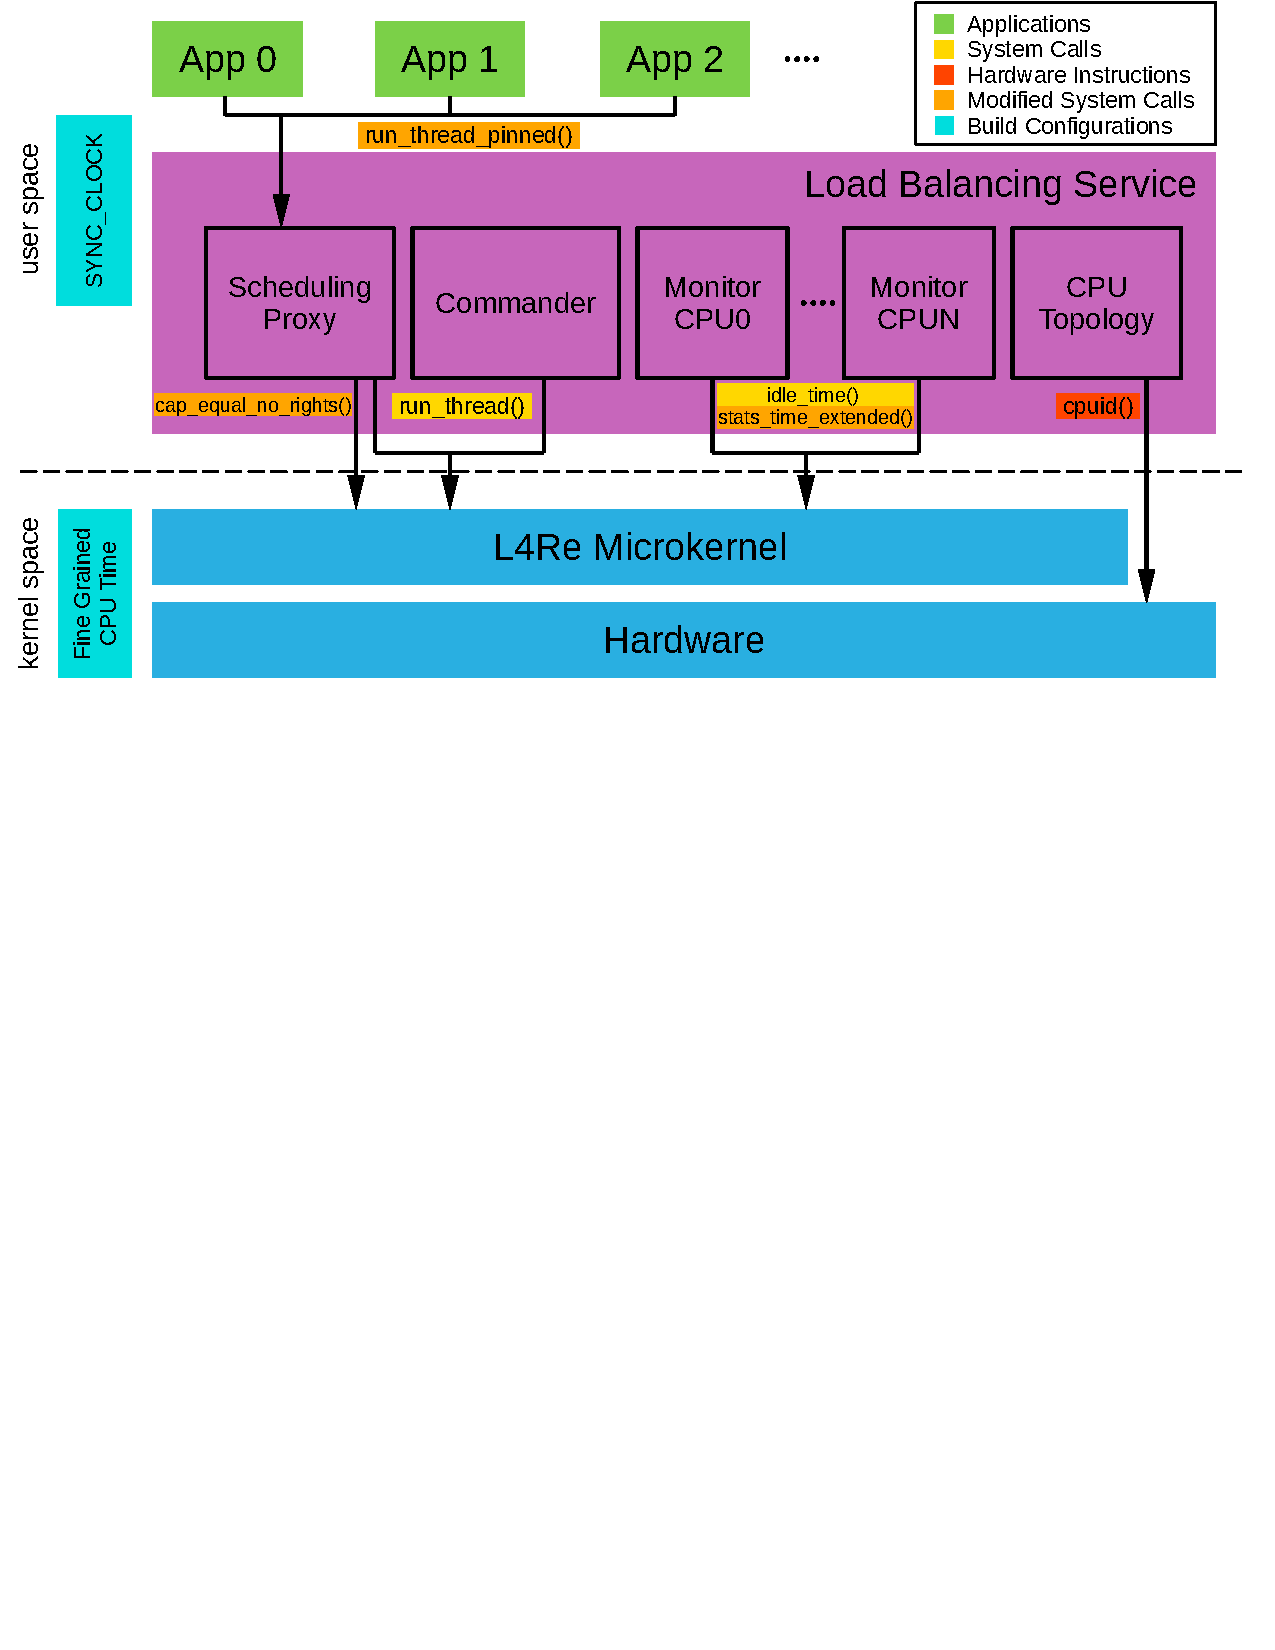
\includegraphics[trim={0 16.5cm 0.3cm 0}, clip, width=\textwidth]{images/arch_overview_impl.pdf}
	\caption{Architecture diagram after the implementation phase. Highlighting modified system calls and required build configurations (compare to Figure~\ref{fig:des:overview}).}
	\label{fig:impl:overview}
\end{figure}

The scheduling proxy (see Section~\ref{sec:proxy}) solved the thread registration process via the extension of the \texttt{cap\_equal()} system call to \texttt{cap\_equal\_no\_rights()}.
During the implementation of the monitoring infrastructure in Section~\ref{sec:monitoring}, the deregistration of dead threads and the probing of live ones were solved by extending \texttt{stats\_time()} to \texttt{stats\_time\_extended()}.
This extension makes the monitor able to read the CPU usage, thread state, and preemption history of a thread.
Additionally, the essential user land and kernel build configurations of \texttt{SYNC\_CLOCK} and \texttt{Fine Grained CPU Time} were added in turquoise in Figure~\ref{fig:impl:overview} as 'Build Configurations'.
In Section~\ref{sec:impl:loba}, thread placement is built on top of the \texttt{vload} metric that is derived from the preemption history of a thread.
Shared data structures like the thread groups that are used for placement constraints required thread-safe access patterns as well as the introduction of the \texttt{run\_thread\_pinned()} call.
As the whole service is implemented in userland, it requires a concurrent distributed system view of the design discussed in Section~\ref{sec:distributed-system}, leading to an alternate parallelization variant to calculate virtual load.
In Section~\ref{sec:l4re-particularities} discusses particularities with main components of the L4Re framework and migration behavior that introduce unavoidable latency.
Both the user of the load balancer and the developer maintaining it need to be aware of this behavior.
The chapter lastly explores optimization paths to reduce the runtime of the monitoring and rebalancing process, making use of parallelism in system calls or avoiding slowdowns caused by hardware components that do not necessarily need to be used, as discussed in Section~\ref{sec:impl:optimizations}.

\cleardoublepage

%%% Local Variables:
%%% TeX-master: "diplom"
%%% End:

\chapter{Evaluation}
\label{sec:evaluation}

% Zu jeder Arbeit in unserem Bereich gehört eine Leistungsbewertung. Aus
% diesem Kapitel sollte hervorgehen, welche Methoden angewandt worden,
% die Leistungsfähigkeit zu bewerten und welche Ergebnisse dabei erzielt
% wurden. Wichtig ist es, dem Leser nicht nur ein paar Zahlen
% hinzustellen, sondern auch eine Diskussion der Ergebnisse
% vorzunehmen. Es wird empfohlen zunächst die eigenen Erwartungen
% bezüglich der Ergebnisse zu erläutern und anschließend eventuell
% festgestellte Abweichungen zu erklären.

The following chapter presents the measurement setup and the final benchmarks used for this thesis and the test cases they were used in as well as a discussion of the results.
The implemented load balancer is compared to the Linux EEVDF scheduler and also measured for overhead and scalability in different configurations.

\section{Measurement Setup and Benchmarks}

\paragraph{Hardware.}

The load balancing component is tested on the Intel Core i9-13900K, a processor with 32 hardware threads.
It follows the Intel hybrid architecture mentioned in Section~\ref{sec:amp}, with eight performance cores that have two hardware threads each and 16 efficiency cores housing one hardware thread.
Additionally, this server has access to 128 GB of DDR5 main memory clocked at \SI{3600}{\mega\hertz}.

\paragraph{Operating System Comparison.}
\label{sec:os-comparison}

The implementation is tested against the well-engineered Linux scheduler; that means that the benchmarks used need to behave similarly on both operating systems.
Hence, established benchmarks are used to construct multiple test cases that can be compared across the boundaries of operating systems.
One problem is that operating systems are complex programs that are made up of more than just a scheduler.
Therefore, multiple components have an influence on execution speed next to the scheduler.

\paragraph{Algorithms.}

The strategies tested during the evaluation are the native L4Re microkernel scheduler, the developed load balancer in two versions, and the Linux EEVDF scheduler.
The first developed version does no periodic balancing but statically assigns a new thread the CPU with the lowest current \texttt{vload} and is therefore static as it operates in 100 \si{\ms} monitoring intervals; it will be referred to as STA100 from now on.
The second variant of the load balancer also includes rebalancing as described in Section~\ref{sec:rebalancing}.
Although both versions make use of the CPU performance scaling explained in Section~\ref{sec:cpu-performance}, the second version will be referred to as AMP.
The AMP balancer is also tested with multiple intervals of the monitoring period (10, 20, 50, 100 \si{\ms}); these will be referenced as AMP<N> with N being the duration of the interval.

\section{SPEC CPU Benchmarks}

The SPEC CPU benchmarking suites\footnote{\url{https://www.spec.org/cpu}} are an established framework to benchmark the hardware it is tested on.
SPEC aims to design benchmarks that try to represent real-world workloads.
Therefore, choosing unique instances from their suites to combine them into test cases that represent real-world scenarios is straightforward.
The SPEC CPU benchmarks were regarded for this work because they are well-tested and already used in previous work done in the field by Eppelt~\cite{philipp-thesis}.

\subsection{SPEC CPU 2006}

The SPEC CPU 2006 benchmark suite\footnote{\url{https://www.spec.org/cpu2006}} contains four tests that cover a wide range of use cases.
Namely, \texttt{403.gcc} representing compiler tasks based on integer computation, \texttt{429.mcf} calculating combinatorial optimization through integers, \texttt{462.libquantum} executing quantum physics integer calculations, and \texttt{470.lbm} doing fluid dynamics based on floating-point operations.
Although the suite is retired and therefore could seem outdated, this fact does not pose a problem, as the benchmarking tests the load balancer, its overhead, and decision-making instead of targeting the hardware.
Additionally, the hardware demands of up to one GB per instance allowed for a significant number of instances at once on the given hardware.

\paragraph{Infeasibility.}

In Section~\ref{sec:cpu0-problem}, it was discussed that freeing memory in L4Re is the task of Moe because it needs to unmap all pages.
With every SPEC CPU 2006 instance occupying up to one GB of main memory according to their specification.
When done in 4 KiB pages, this leads to thousands of pages that need to be unmapped when a single instance finishes execution, monopolizing CPU0 in the process.
This alone is suboptimal, but those benchmarks verify their computation by printing information to serial output; every thread was additionally waiting for its \texttt{printf()} calls to be handled as well.
This behavior results in every thread on every CPU waiting for Moe on CPU0 to become available and handle either their memory unmapping or their standard output.
Finally defeating the purpose of having independent processing instances that need to be scheduled because the bottleneck of the system is the handling of serial output and not the efficiency of the load balancing service developed throughout this thesis.

\subsection{SPEC CPU 2017}

The 2017 suite\footnote{\url{https://www.spec.org/cpu2017}} of SPEC CPU provides three out of the four benchmarks chosen from the 2006 suite.
Therefore, the updated versions \texttt{505.mcf\_r} and \texttt{519.lbm\_r} were ported to the L4Re environment.

\paragraph{Infeasibility.}

Unfortunately, a single instance of these benchmarks runs for almost 10 minutes making it unsuitable for multi threaded execution despite the memory unmapping problem. This also makes the latest release of the SPEC CPU 2026 suite infeasible, because it has the same 2 GB memory requirements per thread and is expected to have an even longer runtime than its 2017 predecessor. 

\section{Used Benchmarks}
\label{sec:bench-used}

The aim was still to cover a wide range of real-world workloads, leading to benchmarks being selected that have comparable characteristics to the SPEC CPU 2006 benchmarks.
The four programs being ported to L4Re ended up being CoreMark\footnote{\url{https://github.com/eembc/coremark}}, STREAM\footnote{\url{https://www.cs.virginia.edu/stream/FTP/Code}}, Whetstone\footnote{\url{https://www.netlib.org/benchmark/whetstone.c}}, and tinymembench\footnote{\url{https://github.com/ssvb/tinymembench}}.
CoreMark performs integer computation and function calls, STREAM tests pointer chasing, Whetstone covers floating-point and math operations, and tinymembench measures memory bandwidth and latency.
All these benchmarks were be ported to L4Re and Linux, making them suitable for the scope of this work.
Unfortunately, STREAM and tinymembench suffer from the same problem as the SPEC CPU benchmarks, although their memory usage got reduced below 10 MB.
Leaving only CoreMark and Whetstone for the final validation runs.

\paragraph{Modifications.}

To avoid thread blocking of the benchmark instances, the serial output in the benchmarks is disabled (see Section~\ref{sec:cpu0-problem}).
CoreMark has an \texttt{ITERATIONS} parameter that was set to \texttt{1'000'000}.
Similarly, Whetstone has its \texttt{LOOP} count set to \texttt{100'000} in combination with the iteration value \texttt{II} with \texttt{100}.
Both these modifications ensure that the benchmarks run for a sufficient and similar time.

\section{Test Cases}
\label{sec:test-cases}

\paragraph{Baseline.}

For this test, a benchmark is run single-threaded sequentially until 100 instances are reached.
The scheduler should only need to decide once on which CPU the single instance is to be executed.
The baseline sets an anchor point to compare the results of following test cases.
It also allows for the usage of the native L4Re scheduler, as it will always schedule any thread on CPU0 that does not have a specific CPU set passed along with it.
Further, it helps to expose differences in execution speeds caused by Linux or L4Re, which are not related to the scheduler.
The investigated schedulers are the native L4Re kernel scheduler, STA100, AMP100, and Linux EEVDF.

\paragraph{CPU Scalability.}

This scenario investigates the scalability of schedulers by assigning them the same numbers of CoreMark threads as they have CPUs to distribute them until 100 instances are finished.
The number of parallel threads and CPUs used are 2, 4, and 8.

\begin{figure}
	\centering
	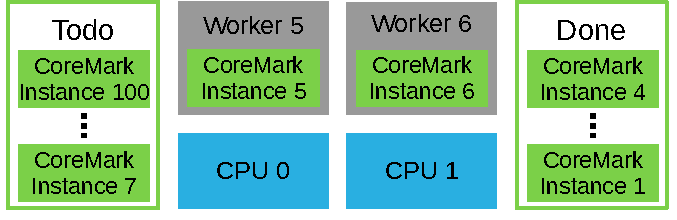
\includegraphics[width=0.7\textwidth]{images/cpu_scaling.pdf}
	\caption{CPU scalability test for two parallel worker threads and two CPUs with 100 CoreMark instances to be computed. Four instances are already done, two are being processed, and 94 need to be spawned and done.}
	\label{fig:cpu-scalability}
\end{figure}


This test represents workloads that can be executed multithreaded.
A common example is the compiler program \texttt{make} used with the additional option of \texttt{-jN}, where N is the number of parallel jobs that are started to finish the compilation.
The investigated schedulers are the static balancer, all four AMP variants, and Linux EEVDF.

\paragraph{Parallel Execution.}

The effect of a well-designed load balancing algorithm shows the most when stressed to the extent of its capabilities.
To mimic this, the parallel execution test contains three cases simulating low, full, and overload by running 8, 16, and 64 instances of each of the CoreMark and Whetstone benchmarks in parallel until 100 instances are finished for each.
To keep the CPU load up consistently at all times, new threads are spawned even when one benchmark reaches its target count until the slower of the two benchmarks finishes its 100 instances.
All three cases test the same schedulers as were already investigated in the CPU scalability scenario.

\paragraph{Monitoring Scalability.}

During the monitoring scalability tests, no benchmarks were used but a custom benchmarking harness for the AMP balancer.
It captures the execution times of the scheduling proxy, commander, and monitors of the AMP balancer with all its four monitoring periods.
Additionally, it tests if the parallel (AMP<N>P) approach to \texttt{vload} updates is superior to the centralized (AMP<N>C) solution argued in Section~\ref{sec:vload-updates}.
All configurations are tracked during the monitoring of 0, 10, 100, 500, 1000, and 2000 idle threads; the spawning parent thread, ITAS, and an additional thread called the pthread manager for a duration of \SI{100}{\second}.
The data points for 0 idle threads are similar to 10 idle threads and are therefore left out for plot readability.
The pthread manager is only spawned whenever the application's main thread spawns at least one additional thread.

\section{Results}

This section presents the results of the benchmarks specified in Section~\ref{sec:bench-used} with their corresponding modifications run in the test cases of Section~\ref{sec:test-cases}.
Further plots of the benchmarks' execution times can be found in Section~\ref{sec:appendix}.

\paragraph{Box Plots.}

As a means of visualizing the 100 single runs of the CoreMark and Whetstone, benchmark box plots were used.
They provide a compact visualization of a data set's distribution by summarizing it through six components. 
The first quartile ($Q_1$) represents the value below which 25\,\% of the data points fall, marking the bottom edge of the box.
Second, the median ($Q_2$) it marks the middle value of the data set, drawn as a line inside the box.
The third quartile ($Q_3$) is the value below which 75\,\% of the data points fall, marking the top edge of the box.
The smallest value in the data set that falls within the lower whisker bound (typically $Q_1 - 1.5 \cdot \text{IQR}$) is called the minimum.
Vice versa, the maximum is the largest value within the upper whisker bound ($Q_3 + 1.5 \cdot \text{IQR}$).
Finally, the outliers mark individual data points lying outside the whisker bounds, plotted separately as distinct markers.
The box itself spans the interquartile range (IQR), that is, $Q_3 - Q_1$, and thus contains the middle 50\,\% of all measured runs.
The whiskers extend to the most extreme data points that still lie within $1.5 \cdot \text{IQR}$ of the box edges, whereas any values beyond this range are flagged as outliers.

\subsection{Baseline}
\label{sec:baseline}

It is important to note that outliers are defined relative to the spread of the bulk of the data, not in absolute terms.
Because the whisker bounds scale with the IQR, a data set with a small IQR will flag comparatively small absolute deviations as outliers, simply because they lie far outside this narrow, consistent range.
As a consequence, a high number of outliers in a box plot does not necessarily indicate a high absolute deviation in the underlying measurements.

\begin{figure}[htbp]
	\centering
	\begin{tikzpicture}
		\begin{groupplot}[
			group style={
				group size=2 by 2,
				horizontal sep=1.2cm,
				vertical sep=0.6cm,
			},
			baseline boxplot,
			legend to name=baselinelegend,
			legend style={font=\small, legend columns=-1},
			]
			
			% CoreMark Baseline
			\nextgroupplot[ylabel={Time [s]}, xlabel={CoreMark Benchmark}]
			\addplot+[boxplot, mark=triangle, color=Orange]  table[y index=0] {data/base/base_fiasco_core.dat};
			\addplot+[boxplot, mark=asterisk, color=BlueGreen]  table[y index=0] {data/base/base_static_core.dat};
			\addplot+[boxplot, mark=+, color=OrangeRed]  table[y index=0] {data/base/base_amp10_core.dat};
			\addplot+[boxplot, mark=Mercedes star, color=ForestGreen]  table[y index=0] {data/base/base_amp20_core.dat};
			\addplot+[boxplot, mark=x, color=Cerulean]  table[y index=0] {data/base/base_amp50_core.dat};
			\addplot+[boxplot, mark=Mercedes star flipped, color=Plum, solid]  table[y index=0] {data/base/base_amp100_core.dat};
			
			\nextgroupplot[width = 2.42cm]
			\addplot+[boxplot, mark=star, color=Goldenrod] table[y index=0] {data/base/base_linux_core.dat};
			
			% Whetstone Baseline
			\nextgroupplot[ylabel={Time [s]}, xlabel={Whetstone Benchmark}]
			\addplot+[boxplot, mark=triangle, color=Orange]  table[y index=0] {data/base/base_fiasco_whet.dat};
			\addplot+[boxplot, mark=asterisk, color=BlueGreen]  table[y index=0] {data/base/base_static_whet.dat};
			\addplot+[boxplot, mark=+, color=OrangeRed]  table[y index=0] {data/base/base_amp10_whet.dat};
			\addplot+[boxplot, mark=Mercedes star, color=ForestGreen]  table[y index=0] {data/base/base_amp20_whet.dat};
			\addplot+[boxplot, mark=x, color=Cerulean]  table[y index=0] {data/base/base_amp50_whet.dat};
			\addplot+[boxplot, mark=Mercedes star flipped, color=Plum, solid]  table[y index=0] {data/base/base_amp100_whet.dat};
			
			\nextgroupplot[width = 2.42cm]
			\addlegendimage{boxplot, mark=triangle, color=Orange}
			\addlegendimage{boxplot, mark=asterisk, color=BlueGreen}
			\addlegendimage{boxplot, mark=+, color=OrangeRed}
			\addlegendimage{boxplot, mark=Mercedes star, color=ForestGreen}
			\addlegendimage{boxplot, mark=x, color=Cerulean}
			\addlegendimage{boxplot, mark=Mercedes star flipped, color=Plum}
			\addplot+[boxplot, mark=star, color=Goldenrod] table[y index=0] {data/base/base_linux_whet.dat};
			\legend{Fiasco, STA100, AMP10, AMP20, AMP50, AMP100, EEVDF}
		\end{groupplot}
		\node[anchor=north] at (current bounding box.south) {\ref{baselinelegend}};
	\end{tikzpicture}
	\caption{Baseline runtimes of the CoreMark (top) and Whetstone (bottom) benchmarks.}
\label{fig:baseline-runtime}
\end{figure}

The baseline runtime provides the minimal execution time of each benchmark as they are run single-threaded with no other load on the system.
The solo execution time serves the purpose of normalizing the results of the upcoming sections because the benchmark itself is not the target of evaluation, but rather the balancing algorithms employed to run them.
Figure~\ref{fig:baseline-runtime} shows on the left for the CoreMark benchmark that the L4Re kernel scheduler has the fastest execution time, closely followed by the STA100 and AMP100 balancer.
The Linux EEVDF scheduler reaches the slowest execution time because an entirely different operating system is being measured, as explained in Section~\ref{sec:os-comparison}.
Those differences become even more apparent when looking at the run-times of the Whetstone benchmark in the same figure on the right-hand side.
EEVDF is trailing by roughly $8.5$ seconds compared to the scheduling services running on the L4Re operating system framework that are all within one hundredth of a second.  

\subsection{CPU Scalability}
\label{sec:cpu-scalability}

Although the test case of CPU scalability (see Section~\ref{sec:test-cases}) is a rather simple one because the optimal solution is to run one thread per CPU, it already exposes the main weakness of the load balancers developed in this thesis.
Figure~\ref{fig:cpun-runtime} shows on the left that EEVDF finishes the 100 CoreMark instances the fastest, followed by all AMP variants, all three finishing within a \SI{10}{\second} window, and lastly, STA100, which takes at least a fifth longer than the others.

\begin{figure}
	\centering
	\subfloat{{
	\begin{tikzpicture}
		\begin{axis}[cpu plot, ylabel = {Time [s]}, ymin = 0]
			\addplot+[fill=BlueGreen,   draw=black] coordinates {(2,2707.0603) (4,1232.0960) (8,761.8451)};
			\addplot+[fill=OrangeRed,   draw=black] coordinates {(2,1955.1869) (4, 990.7111) (8,508.7435)};
			\addplot+[fill=ForestGreen, draw=black] coordinates {(2,1956.5676) (4, 980.1470) (8,509.7714)};
			\addplot+[fill=Cerulean,    draw=black] coordinates {(2,1965.1045) (4, 981.2328) (8,509.5334)};
			\addplot+[fill=Plum,        draw=black] coordinates {(2,1965.4307) (4, 981.8653) (8,500.3606)};
			\addplot+[fill=Goldenrod,   draw=black] coordinates {(2,1822.7732) (4, 911.0701) (8,464.3705)};
			\legend{STA100, AMP10, AMP20, AMP50, AMP100, EEVDF}
		\end{axis}
	\end{tikzpicture}
	}}
	\hfill
	\subfloat{{
	\begin{tikzpicture}
		\begin{axis}[cpu plot, ylabel = {Baseline / Time}, ymin = 0.4, ymax = 1.0]
			\addplot+[fill=BlueGreen,   draw=black] coordinates {(2,0.5334) (4,0.5860) (8,0.4928)};
			\addplot+[fill=OrangeRed,   draw=black] coordinates {(2,0.7386) (4,0.7288) (8,0.7380)};
			\addplot+[fill=ForestGreen, draw=black] coordinates {(2,0.7405) (4,0.7390) (8,0.7389)};
			\addplot+[fill=Cerulean,    draw=black] coordinates {(2,0.7351) (4,0.7361) (8,0.7371)};
			\addplot+[fill=Plum,        draw=black] coordinates {(2,0.7351) (4,0.7357) (8,0.7508)};
			\addplot+[fill=Goldenrod,   draw=black] coordinates {(2,0.7995) (4,0.7998) (8,0.8159)};
		\end{axis}
	\end{tikzpicture}
	}}
	\caption{Absolute runtime (left) and runtime normalized against baseline (right), by CPU count.}
\label{fig:cpun-runtime}
\end{figure}

The explanation for this behavior is distributed system design.
The scheduling proxy has to select a CPU for a thread in \texttt{run\_thread} based on the latest \texttt{vload} information.
The virtual load is (in this version) calculated by the commander.
In future versions the computation should be parallelized and done by the monitors as explained in Section~\ref{sec:vload-updates}; however, this approach would also suffer the same inconvenience.
When the proxy adds a new thread to its run queues, the \texttt{vload} on that CPU is not raised immediately.
Hence, when multiple threads are added in rapid succession, the inertia of virtual load leads to multiple threads being moved to the same CPU because it seems not loaded, resulting in a so-called pile-on.
The AMP variants suffer the same problem, but they can mitigate this effect by rebalancing.

The right side of Figure~\ref{fig:cpun-runtime} visualizes the relative speed compared to the minimum possible runtime reached by baseline execution times.
Note that the y-axis is scaled to an interval of 0.4 to 1.
Those results need to be evaluated with caution because additional resource contention inflates total execution time relative to the theoretical minimum.
EEVDF reaches the highest with 80.5\,\% on average, which does not mean that the Linux scheduler has an overhead of almost 20\,\%.
The STA100 balancer swings between 49 and 59\,\%, demonstrating that execution times vary drastically depending on how excessive the pile-on is.
The AMP versions finish between 73 and 75\,\%.
Those results are a lot more consistent than the ones of STA100, but they first have to get rid of the potential pile-on by rebalancing, introducing more overhead than necessary.
The results also reflect the amount of time and resources that went into the development of the Linux scheduler to overcome the Pareto Principle~\cite{pareto_principle}, also known as the 80:20 rule.

\subsection{Parallel Execution}
\label{sec:para-execution}

As already mentioned in Section~\ref{sec:test-cases}, the true value of a load balancer becomes apparent under high stress.
Figure~\ref{fig:para-runtime} presents similar results to the ones shown in Section~\ref{sec:cpu-scalability}.
The STA100 balancer again suffers from the previously mentioned problem and hence has the slowest execution times.
In the three test cases it reaches roughly 2.5 to 4 times the execution time compared to the other balancers.
EEVDF has a higher runtime than the four AMP balancer services, not because of load distribution but because Linux has a longer runtime for both benchmarks (see Section~\ref{sec:baseline}).
For the four AMP configurations developed in this thesis, AMP20 has a slight edge over the other three, which finish 0.3 to 5.8\,\% behind across all test cases.

\begin{figure}[htbp]
	\centering
	\subfloat{{
	\begin{tikzpicture}
		\begin{axis}[para plot,	ylabel = {Time [s]}, ymin = 0]
			\addplot+[fill=BlueGreen,   draw=black] coordinates {(Under,1265.4084) (Full,971.4656) (Over,754.5777)};
			\addplot+[fill=OrangeRed,   draw=black] coordinates {(Under, 457.5612) (Full,250.8342) (Over,308.5090)};
			\addplot+[fill=ForestGreen, draw=black] coordinates {(Under, 443.1045) (Full,240.8708) (Over,305.0157)};
			\addplot+[fill=Cerulean,    draw=black] coordinates {(Under, 454.5563) (Full,241.6868) (Over,322.5399)};
			\addplot+[fill=Plum,        draw=black] coordinates {(Under, 446.0036) (Full,246.8622) (Over,307.1365)};
			\addplot+[fill=Goldenrod,   draw=black] coordinates {(Under, 521.9691) (Full,295.1491) (Over,359.5003)};
			\legend{STA100, AMP10, AMP20, AMP50, AMP100, EEVDF}
		\end{axis}
	\end{tikzpicture}
	}}
	\hfill
	\subfloat{{
	\begin{tikzpicture}
		\begin{axis}[para plot, ylabel = {Baseline / Time},	ymin = 0.1,	ymax = 1]
			\addplot+[fill=BlueGreen,   draw=black] coordinates {(Under,0.2967) (Full,0.2230) (Over,0.3674)};
			\addplot+[fill=OrangeRed,   draw=black] coordinates {(Under,0.8206) (Full,0.8636) (Over,0.8987)};
			\addplot+[fill=ForestGreen, draw=black] coordinates {(Under,0.8501) (Full,0.9022) (Over,0.9119)};
			\addplot+[fill=Cerulean,    draw=black] coordinates {(Under,0.8262) (Full,0.8965) (Over,0.8599)};
			\addplot+[fill=Plum,        draw=black] coordinates {(Under,0.8423) (Full,0.8779) (Over,0.9032)};
			\addplot+[fill=Goldenrod,   draw=black] coordinates {(Under,0.8978) (Full,0.9160) (Over,0.9626)};
		\end{axis}
	\end{tikzpicture}
	}}
	\caption{Absolute runtime (left) and runtime normalized against baseline (right), by processor load.}
	\label{fig:para-runtime}
\end{figure}

The right side of Figure~\ref{fig:para-runtime} shows the same runtimes normalized against the theoretically minimal runtime derived from the baseline measurements.
Note that the y-axis is scaled to an interval of 0.1 to 1, and resource contention under parallel execution inflates the total runtime beyond the theoretical minimum, so these values should not be read as a direct overhead measurement.
EEVDF again achieves the closest approach to baseline, reaching 89.8, 91.6, and 96.3\,\% in the under-, full-, and overload scenarios.
The four AMP variants trail slightly behind, clustering between 82.1 and 91.2\,\% across all three load levels, a narrower and more consistent band than the one observed in the CPU scalability results, with AMP20 again holding a small edge consistent with the absolute runtimes previously discussed.
STA100 again performs the worst by a wide margin, reaching only 22.3 to 36.7\,\% of baseline.
The effect is even more pronounced here than in Section~\ref{sec:cpu-scalability}.
Under sustained parallel load, more threads are dispatched to the scheduling proxy in quick succession, which compounds the pile-on problem described previously.

\subsection{Monitoring Scalability}
\label{sec:overhead-analysis}

As explained in Section~\ref{sec:test-cases}, this section evaluates the performance gains by the changes introduced in Section~\ref{sec:vload-updates}.
The centralized calculation of \texttt{vload} values takes up between 52\,\% and 73\,\% of the total time consumed by the commander and monitor loop (averaged over all monitoring intervals).
Amdahl's law describes the theoretical speedup $S$ achievable through parallelization as $S = \frac{1}{(1-P)+\frac{P}{32}}$, where $P$ is the proportion of the program's execution that can be run in parallel, and 32 corresponds to the maximum number of parallel execution units available in this evaluation~\cite{amdahls_law}.
The values of $P$ observed in this work result in a theoretical speedup between 2.01 and 3.40.

\begin{figure}[htbp]
	\centering
	\begin{tikzpicture}
		\begin{groupplot}[
			group style = {
				group size = 1 by 3,
				xlabels at = edge bottom,
				xticklabels at = edge bottom,
				vertical sep = 0.3cm,
			},
			overhead plot,
			legend to name = overheadlegend,
			legend style = {font=\small, legend columns=1},
			]
			
			% Plot 1: run_thread
			\nextgroupplot[ylabel = {proxy}]
			\addplot+[color=OrangeRed,   solid,  mark=o]          table[x=threads,y=AMP10C]  {data/abs/run_thread_avg.dat};
			\addplot+[color=OrangeRed,   dashed, mark=triangle*]  table[x=threads,y=AMP10P]  {data/abs/run_thread_avg.dat};
			\addplot+[color=ForestGreen, solid,  mark=o]          table[x=threads,y=AMP20C]  {data/abs/run_thread_avg.dat};
			\addplot+[color=ForestGreen, dashed, mark=triangle*]  table[x=threads,y=AMP20P]  {data/abs/run_thread_avg.dat};
			\addplot+[color=Cerulean,    solid,  mark=o]          table[x=threads,y=AMP50C]  {data/abs/run_thread_avg.dat};
			\addplot+[color=Cerulean,    dashed, mark=triangle*]  table[x=threads,y=AMP50P]  {data/abs/run_thread_avg.dat};
			\addplot+[color=Plum,        solid,  mark=o]          table[x=threads,y=AMP100C] {data/abs/run_thread_avg.dat};
			\addplot+[color=Plum,        dashed, mark=triangle*]  table[x=threads,y=AMP100P] {data/abs/run_thread_avg.dat};
			
			% Plot 2: monitor
			\nextgroupplot[ylabel = {monitor}]
			\addplot+[color=OrangeRed,   solid,  mark=o]          table[x=threads,y=AMP10C]  {data/abs/monitor_loop_avg.dat};
			\addplot+[color=OrangeRed,   dashed, mark=triangle*]  table[x=threads,y=AMP10P]  {data/abs/monitor_loop_avg.dat};
			\addplot+[color=ForestGreen, solid,  mark=o]          table[x=threads,y=AMP20C]  {data/abs/monitor_loop_avg.dat};
			\addplot+[color=ForestGreen, dashed, mark=triangle*]  table[x=threads,y=AMP20P]  {data/abs/monitor_loop_avg.dat};
			\addplot+[color=Cerulean,    solid,  mark=o]          table[x=threads,y=AMP50C]  {data/abs/monitor_loop_avg.dat};
			\addplot+[color=Cerulean,    dashed, mark=triangle*]  table[x=threads,y=AMP50P]  {data/abs/monitor_loop_avg.dat};
			\addplot+[color=Plum,        solid,  mark=o]          table[x=threads,y=AMP100C] {data/abs/monitor_loop_avg.dat};
			\addplot+[color=Plum,        dashed, mark=triangle*]  table[x=threads,y=AMP100P] {data/abs/monitor_loop_avg.dat};
			
			% Plot 3: commander
			\nextgroupplot[ylabel = {commander}, xlabel = {Idle Threads}]
			\addplot+[color=OrangeRed,   solid,  mark=o]          table[x=threads,y=AMP10C]  {data/abs/commander_loop_avg.dat};
			\addplot+[color=OrangeRed,   dashed, mark=triangle*]  table[x=threads,y=AMP10P]  {data/abs/commander_loop_avg.dat};
			\addplot+[color=ForestGreen, solid,  mark=o]          table[x=threads,y=AMP20C]  {data/abs/commander_loop_avg.dat};
			\addplot+[color=ForestGreen, dashed, mark=triangle*]  table[x=threads,y=AMP20P]  {data/abs/commander_loop_avg.dat};
			\addplot+[color=Cerulean,    solid,  mark=o]          table[x=threads,y=AMP50C]  {data/abs/commander_loop_avg.dat};
			\addplot+[color=Cerulean,    dashed, mark=triangle*]  table[x=threads,y=AMP50P]  {data/abs/commander_loop_avg.dat};
			\addplot+[color=Plum,        solid,  mark=o]          table[x=threads,y=AMP100C] {data/abs/commander_loop_avg.dat};
			\addplot+[color=Plum,        dashed, mark=triangle*]  table[x=threads,y=AMP100P] {data/abs/commander_loop_avg.dat};
			
			\legend{AMP10C, AMP10P, AMP20C, AMP20P, AMP50C, AMP50P, AMP100C, AMP100P}
		\end{groupplot}
		
		\node[rotate=90, anchor=south] at ($(current bounding box.west)!0.5!(current bounding box.south west) + (0cm,3.05cm)$)
		{Time [\si{\micro\second}]};
		
		\node[anchor=west] at ($(current bounding box.east) + (-0.3cm,0.5cm)$) {\ref{overheadlegend}};
	\end{tikzpicture}
	
	\caption{Average overhead per function across proxy (\texttt{run\_thread()}), monitor (\texttt{monitor\_loop()}), and commander (\texttt{commander\_loop()}) components. The centralized (C) approaches (solid) vs. the parallel (P) implementation (dashed).}
	\label{fig:overhead-combined}
\end{figure}

For the scheduling proxy, the only function worth measuring is \texttt{run\_thread()} because it is called frequently by applications to sign up or reassign threads.
The overhead of reading the CPU topology and benchmarking CPUs to scale their performance was not monitored.
This procedure happens once during the startup of the load balancing service and can therefore be neglected, as no continuous overhead is introduced.
Monitors are regarded with respect to their \texttt{monitor\_loop()} as well as the commander with its \texttt{commander\_loop()}.

The \texttt{run\_thread()} implementation scales linearly with the idle thread count in the first plot of Figure~\ref{fig:overhead-combined}.
Due to the linear scan of all thread capabilities to check if the thread is already tracked or new to the load balancers' run queues, a $\mathcal{O}(n)$ runtime cannot be avoided.
As no change has been made to the function during the parallelization process and it is not called periodically, there is no noticeable difference between the eight implementations, as they are all running on the same source code.

A similar behavior can be observed for the \texttt{monitor\_loop()}, as it also needs to probe threads based on their linearly growing run queues.
Against the intuition that the monitor should take longer for one loop iteration if it additionally needs to compute the \texttt{vload} of its CPU, all parallel approaches represented by dashed lines have a smaller average runtime.
This phenomenon is likely due to cache effects, as the virtual load value is part of the CPU state.
This state is partly updated by the monitor and commander in the centralized solution.
In the parallel approach, the update is entirely done by the monitor and only overwritten by the commander when a monitor is outdated, which happens rarely.
This leads to less cache contention, where individual lines need to be loaded, alternating between different CPUs.
As the monitoring scales linearly and the probing itself takes between 15 and \SI{20}{\micro\second}, the average probing time per thread is about 240 to \SI{320}{\ns}.

Finally, the benefits of parallelization become apparent in the third plot of Figure~\ref{fig:overhead-combined} for the \texttt{commander\_loop()}.
These overhead measurements need to be treated with reservation because idle threads, regardless of count, do not require true rebalancing.
Hence, the results should only be taken for evaluating the speedup due to the shift in \texttt{vload} calculations.
The parallel approaches only increase by 1.6 in runtime when increasing the number of monitored threads from 0 to 2000, and they consistently stay below the \SI{10}{\micro\second} barrier.
As expected, the centralized implementations raise their runtime by 5.3 over the course of increasing idle threads, with all variants breaking the \SI{60}{\micro\second} mark in the end.

\begin{table}
	\centering
	\begin{threeparttable}
		\begin{tabular}{l c c c c}
			\toprule
			Algorithm & Proxy [\%] & Monitor [\%] & Commander [\%] & C/P Speedup\tnote{1} \\
			\midrule
			AMP10C  & 0.000--0.128 & 0.014--0.215 & 0.146--0.764 & --- \\
			AMP10P  & 0.000--0.124 & 0.014--0.187 & 0.055--0.090 & 2.282--3.521 \\
			\addlinespace
			AMP20C  & 0.000--0.123 & 0.006--0.105 & 0.057--0.307 & --- \\
			AMP20P  & 0.000--0.119 & 0.006--0.105 & 0.027--0.045 & 1.914--2.737 \\
			\addlinespace
			AMP50C  & 0.000--0.117 & 0.002--0.042 & 0.023--0.141 & --- \\
			AMP50P  & 0.000--0.116 & 0.003--0.038 & 0.010--0.012 & 1.994--3.600 \\
			\addlinespace
			AMP100C & 0.000--0.118 & 0.001--0.021 & 0.015--0.060 & --- \\
			AMP100P & 0.000--0.117 & 0.001--0.017 & 0.005--0.007 & 2.497--3.406 \\
			\bottomrule
		\end{tabular}
		\begin{tablenotes}
			\item[1] Computed from monitor and commander overhead, as only these two were affected by the change discussed in Section~\ref{sec:vload-updates}.
		\end{tablenotes}
	\end{threeparttable}
	\caption{Percentage overhead of the scheduling proxy, monitor, and commander as well as the speedup gained by the parallelization of the \texttt{vload} calculation.}
	\label{tab:overhead-normalized}
\end{table}


Table~\ref{tab:overhead-normalized} shows the percentage overhead introduced by each component of the load balancer.
They reflect the average run times from Figure~\ref{fig:overhead-combined} partly but take the monitoring interval into account.
The load balancer configured with a lower monitoring period introduces, therefore, a higher overhead.
It is to be noted that the overhead of the monitoring component in Table~\ref{tab:overhead-normalized} is not absolute but for a single CPU.
The proxy overhead remains nearly constant across all configurations and variants (0.000\,\%--0.128\,\%), because it is not dependent on the monitoring interval or the changes discussed in Section~\ref{sec:vload-updates}.
All parallelized monitor variants (0.001\,\%--0.187\,\%) are even with or have a slight edge over their centralized counterparts (0.001\,\%--0.215\,\%).
In combination with the parallelized \texttt{commander\_loop} versions (0.005\,\%--0.090\,\%), they reach a speedup of 1.914--3.600.
This speedup aligns with the previously calculated values of Amdahl's law.
Although it is meant to be an upper bound, the overshoots can be explained by the decrease in execution time of the monitors even though they needed to carry out more instructions.
The presented speedup is only gained for the CPU the commander is located on, as all other CPUs only have one monitor thread to run, except for CPU1, where the scheduling proxy is placed.
The switch to the parallelized version still results in an average system-wide speedup of $\times$1.15 over all monitoring intervals and idle thread counts.

\section{Summary}

The results presented in this chapter allow for a consistent picture of the load balancing service developed throughout this thesis.
STA100, the balancer without periodic rebalancing, is consistently the worst-performing variant across all test cases, most visibly in the CPU scalability (Section~\ref{sec:cpu-scalability}) and parallel execution (Section~\ref{sec:para-execution}) scenarios, where the pile-on effect caused by the inertia of \texttt{vload} regularly costs it between two and four times the runtime of any AMP variant.
Because monitoring the system state is already required to keep track of dead threads, the additional cost of computing \texttt{vload} and rebalancing on it is comparatively small.
STA100 is therefore better characterized as a baseline establishing the value of rebalancing than as a viable configuration in its own right.

Among the four AMP variants, the monitoring interval has only a minor influence on end-to-end performance.
AMP20 holds a small but consistent edge over AMP10, AMP50, and AMP100, finishing within 0.3 to 5.8\,\% of the fastest variant per test case, even though no configuration is uniformly best across all scenarios.
Section~\ref{sec:overhead-analysis} explains why: even AMP10 keeps its per-component overhead under a fraction of a percent of total runtime, and the parallelized \texttt{vload} computation reduces the commander's contribution well below the Amdahl's Law upper bound.

None of the AMP variants close the throughput gap to Linux's EEVDF scheduler.
EEVDF remains fastest in every test case, reaching 80.0\,\% to 96.3\,\% of the theoretical baseline runtime depending on the scenario, with the AMP variants trailing by roughly 2 to 7 percentage points.
On this metric, the developed load balancer does not outperform a scheduler with over a decade of engineering behind it inside a monolithic kernel, an expected outcome given the maturity gap and the constraints of the microkernel's distributed design discussed in Section~\ref{sec:cpu-scalability}.
Additionally, throughput is only one axis of comparison, and the Figures~\ref{fig:cpun-runtime-distr} and~\ref{fig:para-runtime-distr} in the appendix examine execution times at the level of individual threads rather than aggregated completion times.
The AMP balancer trail EEVDF by only small margins overall but shows noticeably higher variance between individual thread completion times under otherwise identical load, where EEVDF's distribution stays considerably tighter.
Taken together, these results position the AMP load balancers as a solid initial approach to running L4Re on asymmetric hardware, with disadvantages that require further refinement.

One methodological limitation of the evaluation should be noted.
All test cases were run until 100 instances of a benchmark had completed (see Section~\ref{sec:test-cases}), a convenient number chosen for readability rather than for compatibility with the parallel test configurations.
The parallel execution scenario spawns 8, 16, and 64 threads concurrently to match the CPU count of the hardware, but 100 is not evenly divisible by any of these counts.
A count of 128 would instead be a multiple of all three parallelism levels, avoiding partial batches and slightly improving comparability.
This inconvenience did not affect the previous conclusions, because additional instances are always spawned to keep system pressure constant until the total count is reached, but it remains a worthwhile adjustment for any follow-up evaluation using the same harness.

\cleardoublepage

%%% Local Variables:
%%% TeX-master: "diplom"
%%% End:

\chapter{Future Work}
\label{sec:futurework}

This chapter explores future directions for the work done in this thesis.
Section~\ref{sec:design-extensions} presents extensions to the current design that would improve the balancing strategy.
This can be achieved either through the adjustment of the policy itself or by incorporating more hardware information into the decision.
In Section~\ref{sec:optimizations}, software optimizations and the efficient use of caches are discussed.

\section{Design Extensions}
\label{sec:design-extensions}

\subsection{Balancing Behavior}

\paragraph{Real-Time Balancing.}

The load balancer is currently following a best-effort policy (see Section~\ref{sec:best-effort}) because it can easily be shown that threads with a high priority will be suspended, although they could run on a different CPU.
This behavior does not preserve the real-time characteristics of the L4Re operating system framework.
Although enabling migrations in a real-time system introduces overhead that must be accounted for in the worst-case execution time, it preserves the assumption that a thread is always able to run when it is technically possible to run it at its given priority.

\paragraph{Fairness.}

Especially when no real-time strategy is employed but rather a best-effort balancer, one optimization goal could be fairness (see Section~\ref{sec:best-effort}).
Currently this goal is not regarded, but it could be added by tracking the time a thread has spent in the system and comparing it to the time it was running.
Doing so, the load balancer could weigh threads of the same priority to receive equal portions of processing time.
A thread could, therefore, receive two kinds of priorities.
The first one being the actual scheduling priority and the second one being a fairness value preferring it over other threads of the same priority when making a migration decision.
This would align with the concept of priority-based scheduling but could avoid cases of unequal processing time, as can be seen in Figure~\ref{fig:para-runtime-distr} of the appendix.

\paragraph{\texttt{Vload} Inertia.}

Section~\ref{sec:cpu-scalability} discusses the phenomenon that the scheduling proxy piles threads onto one CPU during the placement decision in \texttt{run\_thread()}.
It becomes most visible in Figure~\ref{fig:para-runtime-distr} of the appendix in the overload case at the bottom.
The STA100 balancer has a significantly faster execution time for most instances, although the total runtime for all threads is much slower (see Section~\ref{sec:para-execution}).
The first spawned benchmarks are piled onto one CPU, but because there are always 64 instances, the following ones have less-loaded CPUs available for their computation, drastically reducing their runtime.
The asynchronous updates of \texttt{vload} by the commander or monitors introduce an inertial effect for which the proxy has no way of accounting.
The solution to this problem could be to immediately add a default margin to the \texttt{vload} of the CPU at which the new thread is placed.
Although this would solve the problem of outdated virtual load information for the proxy, it could introduce arbitrary changes of \texttt{vload} during the balancing process for the commander.
Further, the solution is also racy in the sense that the proxy addition could immediately be overwritten by the monitor updating the virtual load according to its monitoring cycle, undermining the intended effect.
It remains to be investigated how this problem can be solved in this concurrent distributed load balancer.

\subsection{Hardware Aware Balancing}

\paragraph{Advanced Topology.}

The load balancer presented in this thesis scans the CPU topology to gain information about heterogeneous cores (see Section~\ref{sec:cpu-performance}), but uniform memory access is assumed.
Hence, there is unexplored potential in the topology itself because cache hierarchies are not read and architectures such as NUMA are not regarded.
Utilizing caches and memory bandwidths and being aware of the full hardware structure are crucial for fast and efficient execution because they can make use of the principle of locality.

\paragraph{CPU Performance Scaling.}

The microbenchmark executed during the start up of the load balancer (see Section~\ref{sec:cpu-performance}) tests simple multiplication and addition operations.
However, modern CPUs consist of multiple acceleration units that speed up the processing of different kinds of instructions (FPU, SVE, and SME), but they also allow for parallelism when operating on multiple registers at once (SIMD, SSE, and AVX).
Not only are the current benchmarks insufficient to measure the whole CPU, but additionally, the result of the measurements cannot be represented by a single scaling value.
It would require an enhanced design testing multiple accelerators and further representing them in a scaling vector that represents fine-grained information about different processing units.
It needs to be mentioned that even with a detailed report of every CPU, the performance of each can be scaled by hardware at any time because of power or heat management.
Hence, the gained information does not necessarily apply to the current state of the hardware.

\paragraph{Thread Behavior Awareness.}

The concept of scaling CPU compute performance breaks the AMP structure of the CPU down to a symmetric one.
As stated in Section~\ref{sec:cpu-performance}, this method works against the concept of having AMP in the first place.
The metric of preemptions (see Section~\ref{sec:des:loba}) was originally introduced to categorize whether threads are compute- or input-output heavy.
Only later were they used to calculate \texttt{vload}, inevitably leaving a gap for determining the behavior of a thread.
Having insight into the kind of processing a thread performs becomes consequential when combined with the previously discussed CPU performance scaling.
It enables the load balancer to move a thread with a distinct behavior profile to a CPU that is structurally beneficial for its execution.

\section{Optimizations}
\label{sec:optimizations}

\paragraph{Batched System Call.}

Section~\ref{sec:impl:bached-stats} explains the idea of an extended \texttt{stats\_time} system call that requests multiple thread stats at once.
Next to the decision of where to implement that functionality, it would require a protocol that clarifies the information transfer.
Threads can still be absent from the CPU they are currently probed on because of either exiting entirely or being in migration transit.
The protocol would need to define a system on how to handle such cases.
Further, the scenario of IPC errors would need to be covered.
If a single thread on a CPU cannot be probed, it is negligible, but if up to 30 threads are not probed, it causes inaccuracies during \texttt{vload} calculation.

\paragraph{Capability Comparison.}

The overhead of the thread capability comparison with \texttt{cap\_equal\_no\_rights()} during \texttt{run\_thread()} does not seem severe (see Section~\ref{sec:overhead-analysis}).
However, it can quickly slow down processing done on CPU1 because the system calls for comparing thread capabilities scale linearly with the number of threads.
If there is a high thread count that the load balancer needs to keep track of and threads are rescheduled often, a constant runtime for \texttt{run\_thread()} is desired.
To avoid those system calls, a mechanism is needed that can either compare them in userland or make comparing obsolete.
It is difficult to do so because because, as explained in Section~\ref{sec:impl:cap-slots}, capabilities are just array indices into the capability table rather than the actual object.
Therefore, this problem may be unsolvable for a load balancer running in the user-space environment of L4Re.

\paragraph{Cache Usage.}

This work does not investigate what influence the caching behavior of the load balancer components has on performance.
Caches are one of the prime primitives to make execution fast.
Inefficient cache use can have dramatic effects on processing speed.
If two threads on different CPUs alternately modify the same data, this leads to the cache line being invalidated and reloaded repeatedly.
Additionally, if data structures are not aligned correctly, this can lead to poor performance because of cache bouncing.
The commander and proxy are always working with the data provided by the monitors.
If the commander and proxy were to invalidate the data cached by the monitors, this would yield poor execution speed.
Investigating such behavior and improving it by properly aligning structures in memory as well as coordinating access patterns could potentially result in less overhead introduced by the load balancer.

\cleardoublepage

%%% Local Variables:
%%% TeX-master: "diplom"
%%% End:

\chapter{Conclusion}
\label{sec:conclusion}

%  Schlußfolgerungen, Fragen, Ausblicke

% Dieses Kapitel ist sicherlich das am Schwierigsten zu schreibende. Es
% dient einer gerafften Zusammenfassung dessen, was man gelernt hat. Es
% ist möglicherweise gespickt von Rückwärtsverweisen in den Text, um dem
% faulen aber interessierten Leser (der Regelfall) doch noch einmal die
% Chance zu geben, sich etwas fundierter weiterzubilden. Manche guten
% Arbeiten werfen mehr Probleme auf als sie lösen. Dies darf man ruhig
% zugeben und diskutieren. Man kann gegebenenfalls auch schreiben, was
% man in dieser Sache noch zu tun gedenkt oder den Nachfolgern ein paar
% Tips geben. Aber man sollte nicht um jeden Preis Fragen, die gar nicht
% da sind, mit Gewalt aufbringen und dem Leser suggerieren, wie
% weitsichtig man doch ist. Dieses Kapitel muß kurz sein, damit es
% gelesen wird.

This thesis presented a load balancing service for the L4Re userland on asymmetric hardware.
The AMP awareness was addressed by scaling CPU performance as described in Section~\ref{sec:cpu-performance}.
This mechanism alone is insufficient for balancing threads because it corrects the differences between cores, but it does not indicate how loaded a core already is.
Therefore, a preemption-based virtual load metric was introduced that captures CPU utilization and saturation (see Section~\ref{sec:des:loba}).
Implementing the load balancing component into the L4Re environment required a series of kernel interface extensions for capability comparison (Section~\ref{sec:impl:proxy}), thread probing (Section~\ref{sec:probing}), and pinning threads (Section~\ref{sec:thread-groups}), because a userland application cannot rely on the omniscience an operating system kernel has.
That the load balancer must reside in user space gave rise to problems never encountered by a kernel scheduler.
It is subject to preemption, stale, or partial system-state information, and it requires careful orchestration of the monitor, proxy, and commander threads (see Section~\ref{sec:distributed-system}).

The developed system was compared against Linux's EEVDF scheduler using a custom benchmarking methodology, and various system configurations were additionally measured for runtime overhead with a dedicated benchmarking harness (Chapter~\ref{sec:evaluation}).
The results show that periodic rebalancing is essential.
The static balancer STA100, which placed threads only at creation time without rebalancing them, trailed the rebalancing configurations by two to four times the runtime, whereas for the AMP configurations, the length of the monitoring interval had comparatively little effect on performance.
All rebalancing configurations remained within a narrow window of each other, and their monitoring overheads stayed under a fraction of a percent even at the shortest interval tested.
However, no configuration developed throughout this thesis could match the throughput of EEVDF, which held an edge of two to seven percent over all AMP variants in normalized runtime in Section~\ref{sec:cpu-scalability} and~\ref{sec:para-execution} and produced much lower variance between individual benchmark run times.
This gap is best understood as a consequence of the microkernel philosophy enforced by L4Re and userland balancing under partial information.
The AMP variants are not able to match a kernel scheduler with unrestricted, synchronous, and thorough access to the system state, let alone the years of engineering that went into its development.

The findings of this work show that the mechanism and policy separation central to the design of L4Re does allow for AMP-aware load balancing, with the load balancers developed in this thesis achieving performance close to an established monolithic scheduler.
Additional overhead is introduced for coordinating a userland-implemented, distributed scheduling component.
The evaluation identified a concrete limitation in \texttt{vload} staleness leading to the observed pile-on effects, and Chapter~\ref{sec:futurework} points to directions for mitigating such behavior in the future.

\cleardoublepage

%%% Local Variables:
%%% TeX-master: "diplom"
%%% End:



\appendix
\refstepcounter{chapter}
\addcontentsline{toc}{chapter}{Appendix}
\chapter*{Appendix}

\section{Statement on the use of AI}

During the writing of this thesis, AI-powered tools, namely Claude Chat and LanguageTool, were used to revise and refine the wording of individual text passages. All suggestions generated by the tools were reviewed and either revised or discarded.

\section{Additional Figures}
\label{sec:appendix}

\renewcommand{\topfraction}{0.98}
\renewcommand{\floatpagefraction}{0.9}
\setcounter{topnumber}{2}

\begin{figure}[htbp]
	\centering
	\begin{tikzpicture}
		\begin{groupplot}[
			group style={
				group size=3 by 3,
				horizontal sep=1cm,
				vertical sep=0.6cm,
			},
			baseline boxplot,
			height = 4.51cm,
			legend to name=cpunlegend,
			legend style={font=\small, legend columns=-1},
			]
			
			% 2 CPUs
			\nextgroupplot[width=2.42cm, ylabel={Time [s]}]
			\addplot+[boxplot, mark=asterisk, color=BlueGreen] table[y index=0] {data/cpun/cpu2_static.dat};
			
			\nextgroupplot[width=6cm, xlabel={2 CPUs / Threads}]
			\addplot+[boxplot, mark=+,                     color=OrangeRed]   table[y index=0] {data/cpun/cpu2_amp10.dat};
			\addplot+[boxplot, mark=Mercedes star,         color=ForestGreen] table[y index=0] {data/cpun/cpu2_amp20.dat};
			\addplot+[boxplot, mark=x,                     color=Cerulean]    table[y index=0] {data/cpun/cpu2_amp50.dat};
			\addplot+[boxplot, mark=Mercedes star flipped, color=Plum]        table[y index=0] {data/cpun/cpu2_amp100.dat};
			
			\nextgroupplot[width=2.42cm]
			\addplot+[boxplot, mark=star, color=Goldenrod] table[y index=0] {data/cpun/cpu2_linux.dat};
			
			% 4 CPUs
			\nextgroupplot[width=2.42cm, ylabel={Time [s]}]
			\addplot+[boxplot, mark=asterisk, color=BlueGreen] table[y index=0] {data/cpun/cpu4_static.dat};
			
			\nextgroupplot[width=6cm, xlabel={4 CPUs / Threads}]
			\addplot+[boxplot, mark=+,                     color=OrangeRed]   table[y index=0] {data/cpun/cpu4_amp10.dat};
			\addplot+[boxplot, mark=Mercedes star,         color=ForestGreen] table[y index=0] {data/cpun/cpu4_amp20.dat};
			\addplot+[boxplot, mark=x,                     color=Cerulean]    table[y index=0] {data/cpun/cpu4_amp50.dat};
			\addplot+[boxplot, mark=Mercedes star flipped, color=Plum]        table[y index=0] {data/cpun/cpu4_amp100.dat};
			
			\nextgroupplot[width=2.42cm]
			\addplot+[boxplot, mark=star, color=Goldenrod] table[y index=0] {data/cpun/cpu4_linux.dat};
			
			% 8 CPUs
			\nextgroupplot[width=2.42cm, ylabel={Time [s]}]
			\addplot+[boxplot, mark=asterisk, color=BlueGreen] table[y index=0] {data/cpun/cpu8_static.dat};
			
			\nextgroupplot[width=6cm, xlabel={8 CPUs / Threads}]
			\addplot+[boxplot, mark=+,                     color=OrangeRed]   table[y index=0] {data/cpun/cpu8_amp10.dat};
			\addplot+[boxplot, mark=Mercedes star,         color=ForestGreen] table[y index=0] {data/cpun/cpu8_amp20.dat};
			\addplot+[boxplot, mark=x,                     color=Cerulean]    table[y index=0] {data/cpun/cpu8_amp50.dat};
			\addplot+[boxplot, mark=Mercedes star flipped, color=Plum]        table[y index=0] {data/cpun/cpu8_amp100.dat};
			
			\nextgroupplot[width=2.42cm]
			\addlegendimage{boxplot, mark=asterisk, color=BlueGreen}
			\addlegendimage{boxplot, mark=+, color=OrangeRed}
			\addlegendimage{boxplot, mark=Mercedes star, color=ForestGreen}
			\addlegendimage{boxplot, mark=x, color=Cerulean}
			\addlegendimage{boxplot, mark=Mercedes star flipped, color=Plum}
			\addplot+[boxplot, mark=star, color=Goldenrod] table[y index=0] {data/cpun/cpu8_linux.dat};
			\legend{STA100, AMP10, AMP20, AMP50, AMP100, EEVDF}
		\end{groupplot}
		\node[anchor=north] at (current bounding box.south) {\ref{cpunlegend}};
	\end{tikzpicture}
	\caption{Runtime of the CoreMark benchmark for 2 (top), 4 (middle), or 8 (bottom) CPU parallelism.}
	\label{fig:cpun-runtime-distr}
\end{figure}


\begin{figure}
	\centering
	\begin{tikzpicture}
		\begin{groupplot}[
			group style={
				group size=4 by 3,
				horizontal sep=0.9cm,
				vertical sep=0.65cm,
			},
			baseline boxplot,
			legend to name=paralegend,
			legend style={font=\small, legend columns=-1},
			]

			% LOW CoreMark + Whetstone
			\nextgroupplot[width = 2.36cm, ylabel = {Time [s]}]
			\addplot+[boxplot, mark=asterisk, color=BlueGreen]  table[y index=0] {data/para/low/low_static_core.dat};
			
			\nextgroupplot[width=5.9cm, xlabel = {CoreMark (8 threads)}]
			\addplot+[boxplot, mark=+,                     color=OrangeRed]  table[y index=0] {data/para/low/low_amp10_core.dat};
			\addplot+[boxplot, mark=Mercedes star,         color=ForestGreen]  table[y index=0] {data/para/low/low_amp20_core.dat};
			\addplot+[boxplot, mark=x,                     color=Cerulean]  table[y index=0] {data/para/low/low_amp50_core.dat};
			\addplot+[boxplot, mark=Mercedes star flipped, color=Plum]  table[y index=0] {data/para/low/low_amp100_core.dat};
			\addplot+[boxplot, mark=star, 				   color=Goldenrod]  table[y index=0] {data/para/low/low_linux_core.dat};
			
			\nextgroupplot[width = 2.36cm]
			\addplot+[boxplot, mark=asterisk, color=BlueGreen]  table[y index=0] {data/para/low/low_static_whet.dat};
			
			\nextgroupplot[width=5.9cm, xlabel = {Whetstone (8 threads)}]
			\addplot+[boxplot, mark=+,                     color=OrangeRed]  table[y index=0] {data/para/low/low_amp10_whet.dat};
			\addplot+[boxplot, mark=Mercedes star,         color=ForestGreen]  table[y index=0] {data/para/low/low_amp20_whet.dat};
			\addplot+[boxplot, mark=x,                     color=Cerulean]  table[y index=0] {data/para/low/low_amp50_whet.dat};
			\addplot+[boxplot, mark=Mercedes star flipped, color=Plum]  table[y index=0] {data/para/low/low_amp100_whet.dat};
			\addplot+[boxplot, mark=star, 				   color=Goldenrod]  table[y index=0] {data/para/low/low_linux_whet.dat};

			% MID CoreMark + Whetstone
			\nextgroupplot[width = 2.36cm, ylabel = {Time [s]}]
			\addplot+[boxplot, mark=asterisk, color=BlueGreen]  table[y index=0] {data/para/mid/mid_static_core.dat};
			
			\nextgroupplot[width=5.9cm, xlabel = {CoreMark (16 threads)}]
			\addplot+[boxplot, mark=+,                     color=OrangeRed]  table[y index=0] {data/para/mid/mid_amp10_core.dat};
			\addplot+[boxplot, mark=Mercedes star,         color=ForestGreen]  table[y index=0] {data/para/mid/mid_amp20_core.dat};
			\addplot+[boxplot, mark=x,                     color=Cerulean]  table[y index=0] {data/para/mid/mid_amp50_core.dat};
			\addplot+[boxplot, mark=Mercedes star flipped, color=Plum]  table[y index=0] {data/para/mid/mid_amp100_core.dat};
			\addplot+[boxplot, mark=star, 				   color=Goldenrod]  table[y index=0] {data/para/mid/mid_linux_core.dat};
			
			\nextgroupplot[width = 2.36cm]
			\addplot+[boxplot, mark=asterisk, color=BlueGreen]  table[y index=0] {data/para/mid/mid_static_whet.dat};
			
			\nextgroupplot[width=5.9cm, xlabel = {Whetstone (16 threads)}]
			\addplot+[boxplot, mark=+,                     color=OrangeRed]  table[y index=0] {data/para/mid/mid_amp10_whet.dat};
			\addplot+[boxplot, mark=Mercedes star,         color=ForestGreen]  table[y index=0] {data/para/mid/mid_amp20_whet.dat};
			\addplot+[boxplot, mark=x,                     color=Cerulean]  table[y index=0] {data/para/mid/mid_amp50_whet.dat};
			\addplot+[boxplot, mark=Mercedes star flipped, color=Plum]  table[y index=0] {data/para/mid/mid_amp100_whet.dat};
			\addplot+[boxplot, mark=star, 				   color=Goldenrod]  table[y index=0] {data/para/mid/mid_linux_whet.dat};

			% HIGH CoreMark + Whetstone
			\nextgroupplot[width = 2.36cm, ylabel = {Time [s]}]
			\addplot+[boxplot, mark=asterisk, color=BlueGreen]  table[y index=0] {data/para/hig/hig_static_core.dat};
			
			\nextgroupplot[width=5.9cm, xlabel = {CoreMark (64 threads)}]
			\addplot+[boxplot, mark=+,                     color=OrangeRed]  table[y index=0] {data/para/hig/hig_amp10_core.dat};
			\addplot+[boxplot, mark=Mercedes star,         color=ForestGreen]  table[y index=0] {data/para/hig/hig_amp20_core.dat};
			\addplot+[boxplot, mark=x,                     color=Cerulean]  table[y index=0] {data/para/hig/hig_amp50_core.dat};
			\addplot+[boxplot, mark=Mercedes star flipped, color=Plum]  table[y index=0] {data/para/hig/hig_amp100_core.dat};
			\addplot+[boxplot, mark=star, 				   color=Goldenrod]  table[y index=0] {data/para/hig/hig_linux_core.dat};
			
			\nextgroupplot[width = 2.36cm]
			\addplot+[boxplot, mark=asterisk, color=BlueGreen]  table[y index=0] {data/para/hig/hig_static_whet.dat};
			
			\nextgroupplot[width=5.9cm, xlabel = {Whetstone (64 threads)}]
			\addlegendimage{boxplot, mark=asterisk, color=BlueGreen}
			\addplot+[boxplot, mark=+,                     color=OrangeRed]  table[y index=0] {data/para/hig/hig_amp10_whet.dat};
			\addplot+[boxplot, mark=Mercedes star,         color=ForestGreen]  table[y index=0] {data/para/hig/hig_amp20_whet.dat};
			\addplot+[boxplot, mark=x,                     color=Cerulean]  table[y index=0] {data/para/hig/hig_amp50_whet.dat};
			\addplot+[boxplot, mark=Mercedes star flipped, color=Plum]  table[y index=0] {data/para/hig/hig_amp100_whet.dat};
			\addplot+[boxplot, mark=star, 				   color=Goldenrod]  table[y index=0] {data/para/hig/hig_linux_whet.dat};
			\legend{STA100, AMP10, AMP20, AMP50, AMP100, EEVDF}
		\end{groupplot}
		\node[anchor=north] at (current bounding box.south) {\ref{paralegend}};
	\end{tikzpicture}
	\caption{Runtime of the CoreMark (left) and Whetstone (right) benchmarks for under (8 threads each, top), full (16 threads each, middle), or overload (64 threads each, bottom).}
	\label{fig:para-runtime-distr}
\end{figure}

\cleardoublepage

%%% Local Variables:
%%% TeX-master: "diplom"
%%% End:


%\addchap{Glossar}

% makeglossaries diplom
%\printglossary[style=altlist]
%\printglossary[type=\acronymtype,style=long]

\printbibliography
\iffalse
    % an aid for Kile autocompletion
    \bibliography{own.bib}
\fi

\end{document}
